%************************* MALO2 MACROS  **************************
% FILE NAME: paper.tex
% DATE: 4/15/99, updated 6/1/2003
% CREATED BY: Larry Schumaker
% EMAIL: s@mars.cas.vanderbilt.edu
% WEB: http://www.math.vanderbilt.edu/~schumake/
% ******************************************************************
%
%		For use in preparing papers for
%
%		     AT01 Proceedings, 2000
%
%		 Larry Schumaker (s@mars.cas.vanderbilt.edu)
%********************  INSTRUCTIONS  **********************************

%1. REPLACE xxx by correct information
%2. INSERT body of text in the sections
%3. INSERT references
%4. REMOVE all lines starting with %
%5. RENAME this file "yourname.tex"

%************************ INITIALIZATION ************************

%	 In TEXing your file remember that TEX will be asking for the
%	 file at01.tex, so have it available in the
%	 same directory as this file.
%


\count100= 1
\count101= 10
   %%replace 3 by the number of pages of your paper.

\input malo2.tex
\input epsf.tex
\input lls00.tex  %% Remove the % sign if you want advanced macros
%\draft  \def\updated{xxxx}
   %% Remove the % sign to get a draft version showing assigned labels
   %% This only works if you input lls00.tex


\title{A Family of 4-Point Dyadic High Resolution}
\titwo{Subdivision Schemes}
  %% Replace xxx by your title.
%\titwo{xxx}
  %% If need two lines for title, replace xxx.
\author{Daniel Lemire}
  %% Replace xxx by author names.
%\autwo{xxx}
  %% If you need two lines for authors, replace xxx.

\def\shorttitle{High Resolution Subdivision}
  %% Replace xxx by a short title for the running head.
\def\shortauthor{D. Lemire}
   %% Replace xxx by author names (initials only) for running head

%   ********************** MACROS  ******************************
\hyphenation{Des-lauriers}
%%  Insert your own macros here
\chardef \atcode = \the \catcode `\@
\catcode `\@ = 11
\catcode160=13  \def^^a0{{\bf?}}      % 160 '240, "a0
\catcode161=13  \def^^a1{!`}          % 161 '241, "a1
\catcode162=13  \def^^a2{{\bf?}}      % 162 '242, "a2
\catcode163=13  \def^^a3{\pounds{}}   % 163 '243, "a3
\catcode164=13  \def^^a4{{\bf?}}      % 164 '244, "a4
\catcode165=13  \def^^a5{{\bf?}}      % 165 '245, "a5
\catcode166=13  \def^^a6{$\vert$}        % 166 '246, "a6
\catcode167=13  \def^^a7{\S{}}        % 167 '247, "a7   \S{} ISO-1, 
\catcode168=13  \def^^a8{\"{ }}       % 168 '250, "a8
\catcode169=13  \def^^a9{\copyright{}}% 169, '251, "a9
\catcode170=13  \def^^aa{{\bf?}}      % 170 '252, "aa
\catcode171=13                        % 171 '253, "ab,
%\@ifundefined{lguill}{\def^^ab{$<<$}}{\def^^ab{\lguill}}
\catcode172=13  \def^^ac{{\bf?}}      % 172 '254, "ac
\catcode173=13  \def^^ad{{\bf?}}      % 173 '255 "ad
\catcode174=13  \def^^ae{{\bf?}}      % 174 '256, "ae
\catcode175=13  \def^^af{{\bf?}}      % 175 '257, "af
\catcode176=13  \def^^b0{{\bf?}}      % 176 '260, "b0  ?? \No
\catcode177=13  \def^^b1{$\pm$}       % 177 '261, "b1  ISO-1 plus-minus  
\catcode178=13  \def^^b2{${}^2$}      % 178, '262, "b2
\catcode179=13  \def^^b3{${}^3$}      % 179, '263, "b3
\catcode180=13  \def^^b4{\'{ }}       % 180, '264, "b4
\catcode181=13  \def^^b5{{\bf?}}      % 181, '265, "b5
\catcode182=13  \def^^b6{\P{}}        % 182, '266, "b6
\catcode183=13  \def^^b7{$\cdot$}     % 183, '267, "b7
\catcode184=13  \def^^b8{\c{ }}       % 184, '270, "b8
\catcode185=13  \def^^b9{${}^1$}      % 185, '271, "b9
\catcode186=13  \def^^ba{{\bf?}}      % 186, '272, "ba
\catcode187=13                        % 187, '273, "bb 
%\@ifundefined{rguill}{\def^^bb{$>>$}}{\def^^bb{\rguill}}     
\catcode188=13  \def^^bc{$\frac 1 4$}      % 188, '274, "bc
\catcode189=13  \def^^bd{$\frac 1 2$}      % 189, '275, "bd
\catcode190=13  \def^^be{$\frac 3 4$}      % 190, '276, "be
\catcode191=13  \def^^bf{?`}          % 191, '277, "bf
\catcode192=13  \def^^c0{\`A}         % 192, '300, "c0
%\@ifundefined{@grave@A@grave@}{\def^^c0{\`A}}{\let^^c0=\@grave@A@grave@}
\catcode193=13  \def^^c1{\'A}         % 193, '301, "c1
%\@ifundefined{@acute@A@acute@}{\def^^c1{\'A}}{\let^^c1=\@acute@A@acute@}
\catcode194=13  \def^^c2{\^A}         %  194, '302, "c2
%\@ifundefined{@circflx@A@circflx@}{\def^^c2{\^A}}{\let^^c2=\@circflx@A@circflx@}
\catcode195=13  \def^^c3{\~A}     % 195, '303, "c3
%\@ifundefined{@tileda@A@tilda@}{\def^^c3{\~A}}{\let^^c3=\@tileda@A@tilda@}
\catcode196=13  \def^^c4{\"A}     % 196, '304, "c4
%\@ifundefined{@Umlaut@A@Umlaut@}{\def^^c4{\"A}}{\let^^c4=\@Umlaut@A@Umlaut@}
\catcode197=13  \def^^c5{\AA{}}   % 197, '305, "c5
%\@ifundefined{@A@A@}{\def^^c5{\AA{}}}{\let^^c5=\@A@A@}
\catcode198=13 \def^^c6{\AE{}}    % 198, '306, "c6
%\@ifundefined{@A@E@}{\def^^c6{\AE{}}}{\let^^c6=\@A@E@}
\catcode199=13  \def^^c7{\c{C}}   % 199, '307, "c7
%\@ifundefined{@cedilla@C@cedilla}{\def^^c7{\c{C}}}{\let^^c7=\@cedilla@C@cedilla}
\catcode200=13  \def^^c8{\`E}     % 200, '310, "c8
%\@ifundefined{@grave@E@grave@}{\def^^c8{\`E}}{\let^^c8=\@grave@E@grave@}
\catcode201=13  \def^^c9{\'E}     % 201, '311, "c9
%\@ifundefined{@acute@E@acute@}{\def^^c9{\'E}}{\let^^c9=\@acute@E@acute@}
\catcode202=13  \def^^ca{\^E}     % 202, '312, "ca
%\@ifundefined{@circflx@E@circflx@}{\def^^ca{\^E}}{\let^^ca=\@circflx@E@circflx@}
\catcode203=13  \def^^cb{{\"E}}   % 203, '313, "cb
%\@ifundefined{@Umlaut@E@Umlaut@}{\def^^cb{\"E}}{\let^^cb=\@Umlaut@E@Umlaut@}
\catcode204=13  \def^^cc{\`I}     % 204, '314, "cc
%\@ifundefined{@grave@I@grave@}{\def^^cc{\`I}}{\let^^cc=\@grave@I@grave@}
\catcode205=13  \def^^cd{\'I}     % 205, '315, "cd
%\@ifundefined{@acute@I@acute@}{\def^^cd{\'I}}{\let^^cd=\@acute@I@acute@}
\catcode206=13  \def^^ce{\^I}     % 206, '316, "ce
%\@ifundefined{@circflx@I@circflx@}{\def^^ce{\^I}}{\let^^ce=\@circflx@I@circflx@}
\catcode207=13  \def^^cf{{\"I}}   % 207, '317, "cf
%\@ifundefined{@Umlaut@I@Umlaut@}{\def^^cf{\"I}}{\let^^cf=\@Umlaut@I@Umlaut@}
\catcode208=13  \def^^d0{\rlap{\raise0.3ex\hbox{--}}D}      % 208, '320, "d0
%\@ifundefined{@Eth@}{}{\let^^d0=\@Eth@}
\catcode209=13  \def^^d1{�}       % 209, '321, "d1
%\@ifundefined{@tileda@N@tilda@}{\def^^d1{\~N}}{\let^^d1\@tileda@N@tilda@}
\catcode210=13  \def^^d2{\`O}     % 210, '322, "d2
%\@ifundefined{@grave@O@grave@}{\def^^d2{\`O}}{\let^^d2=\@grave@O@grave@}
\catcode211=13  \def^^d3{\'O}     % 211, '323, "d3
%\@ifundefined{@acute@O@acute@}{\def^^d3{\'O}}{\let^^d3\@acute@O@acute@}
\catcode212=13  \def^^d4{\^O}     % 212, '324, "d4
%\@ifundefined{@circflx@O@circflx@}{\def^^d4{\^O}}{\let^^d4=\@circflx@O@circflx@}
\catcode213=13  \def^^d5{\~O}     % 213, '325, "d5
%\@ifundefined{@tileda@O@tilda@}{\def^^d5{\~O}}{\let^^d5\@tileda@O@tilda@}
\catcode214=13  \def^^d6{\"O}     % 214, '326, "d6
%\@ifundefined{@Umlaut@O@Umlaut@}{\def^^d6{\"O}}{\let^^d6=\@Umlaut@O@Umlaut@}
\catcode215=13  \def^^d7{$\times$}% 215, '327, "d7
\catcode216=13  \def^^d8{\O{}}    % 216, '330, "d8
%\@ifundefined{@OOO@}{\def^^d8{\O{}}}{\let^^d8=\@OOO@}
\catcode217=13  \def^^d9{\`U}     % 217, '331, "d9
%\@ifundefined{@grave@U@grave@}{\def^^d9{\`U}}{\let^^d9=\@grave@U@grave@}
\catcode218=13  \def^^da{\'U}     % 218, '332, "da
%\@ifundefined{@acute@U@acute@}{\def^^da{\'U}}{\let^^da=\@acute@U@acute@}
\catcode219=13  \def^^db{\^U}     % 219, '333, "db
%\@ifundefined{@circflx@U@circflx@}{\def^^db{\^U}}{\let^^db=\@circflx@U@circflx@}
\catcode220=13  \def^^dc{\"U}     % 220, '334, "dc
%\@ifundefined{@Umlaut@U@Umlaut@}{\def^^dc{\"U}}{\let^^dc=\@Umlaut@U@Umlaut@}
\catcode221=13  \def^^dd{{\'Y}}   % 221, '335, "dd
%\@ifundefined{@acute@Y@acute@}{\def^^dd{\'Y}}{\let^^dd=\@acute@Y@acute@}
\catcode222=13  \def^^de{\lower 0.7ex \hbox{l}\hskip-1ex\relax b} % 222, '336, "de
%\@ifundefined{@Thorn@}{}{\let^^de=\@Thorn@}
\catcode223=13  \def^^df{\ss{}}   % 223, '337, "df
%\@ifundefined{@sss@}{\def^^df{\ss{}}}{\let^^df=\@sss@}
\catcode224=13  \def^^e0{\`a}     % 224, '340, "e0
%\@ifundefined{@grave@a@grave@}{\def^^e0{\`a}}{\let^^e0=\@grave@a@grave@}
\catcode225=13  \def^^e1{\'a}     % 225, '341, "e1
%\@ifundefined{@acute@a@acute@}{\def^^e1{\'a}}{\let^^e1=\@acute@a@acute@}
\catcode226=13  \def^^e2{\^a}     % 226, '342, "e2
%\@ifundefined{@circflx@a@circflx@}{\def^^e2{\^a}}{\let^^e2=\@circflx@a@circflx@}
\catcode227=13  \def^^e3{\~a}     % 227, '343, "e3
%\@ifundefined{@tileda@a@tilda@}{\def^^e3{\~a}}{\let^^e3=\@tileda@a@tilda@}
\catcode228=13  \def^^e4{\"a}     % 228, '344, "e4
%\@ifundefined{@Umlaut@a@Umlaut@}{\def^^e4{\"a}}{\let^^e4=\@Umlaut@a@Umlaut@}
\catcode229=13  \def^^e5{\aa{}}   % 229, '345, "e5
%\@ifundefined{@a@a@}{\def^^e5{\aa{}}}{\let^^e5=\@a@a@}
\catcode230=13  \def^^e6{\ae{}}   % 230, '346, "e6
%\@ifundefined{@a@e@}{\def^^e6{\ae{}}}{\let^^e6=\@a@e@}
\catcode231=13  \def^^e7{\c{c}}   % 231, '347, "e7
%\@ifundefined{@cedilla@c@cedilla}{\def^^e7{\c{c}}}{\let^^e7=\@cedilla@c@cedilla}
\catcode232=13  \def^^e8{\`e}     % 232, '350, "e8
%\@ifundefined{@grave@e@grave@}{\def^^e8{\`e}}{\let^^e8=\@grave@e@grave@}
\catcode233=13  \def^^e9{\'e}     % 233, '351, "e9
%\@ifundefined{@acute@e@acute@}{\def^^e9{\'e}}{\let^^e9=\@acute@e@acute@}
\catcode234=13  \def^^ea{\^e}     % 234, '352, "ea
%\@ifundefined{@circflx@e@circflx@}{\def^^ea{\^e}}{\let^^ea=\@circflx@e@circflx@}
\catcode235=13  \def^^eb{\"e}     % 235, '353, "eb
%\@ifundefined{@Umlaut@e@Umlaut@}{\def^^eb{\"e}}{\let^^eb=\@Umlaut@e@Umlaut@}
\catcode236=13  \def^^ec{\`{\i}}  % 236, '354, "ec
%\@ifundefined{@grave@i@grave@}{\def^^ec{\`{\i}}}{\let^^ec=\@grave@i@grave@}
\catcode237=13  \def^^ed{\'{\i}}  % 237, '355, "ed
%\@ifundefined{@acute@i@acute@}{\def^^ed{\'{\i}}}{\let^^ed=\@acute@i@acute@}
\catcode238=13  \def^^ee{\^{\i}}  % 238, '356, "ee
%\@ifundefined{@circflx@i@circflx@}{\def^^ee{\^{\i}}}{\let^^ee=\@circflx@i@circflx@}
\catcode239=13  \def^^ef{\"{\i}}  % 239, '357, "ef
%\@ifundefined{@Umlaut@i@Umlaut@}{\def^^ef{\"{\i}}}{\let^^ef=\@Umlaut@i@Umlaut@}
\catcode240=13  \def^^f0{$\partial$}      % 240, '360, "f0
%\@ifundefined{@eth@}{\def^^f0{$\partial$}}{\let^^f0=\@eth@}
\catcode241=13  \def^^f1{\~n}     % 241, '361, "f1
%\@ifundefined{@tileda@n@tilda@}{\def^^f1{\~n}}{\let^^f1\@tileda@n@tilda@}
\catcode242=13  \def^^f2{\`o}     % 242, '362, "f2
%\@ifundefined{@grave@o@grave@}{\def^^f2{\`o}}{\let^^f2=\@grave@o@grave@}
\catcode243=13  \def^^f3{\'o}     % 243, '363, "f3
%\@ifundefined{@acute@o@acute@}{\def^^f3{\'o}}{\let^^f3\@acute@o@acute@}
\catcode244=13  \def^^f4{\^o}     % 244, '364, "f4
%\@ifundefined{@circflx@o@circflx@}{\def^^f4{\^o}}{\let^^f4=\@circflx@o@circflx@}
\catcode245=13  \def^^f5{\~o}     % 245, '365, "f5
%\@ifundefined{@tileda@o@tilda@}{\def^^f5{\~o}}{\let^^f5\@tileda@o@tilda@}
\catcode246=13  \def^^f6{\"o}     % 246, '366, "f6
%\@ifundefined{@Umlaut@o@Umlaut@}{\def^^f6{\"o}}{\let^^f6=\@Umlaut@o@Umlaut@}
\catcode247=13  \def^^f7{$\div$}   % 247, '367, "f7
\catcode248=13  \def^^f8{\o{}}    % 248, '370, "f8
%\@ifundefined{@ooo@}{\def^^f8{\o{}}}{\let^^f8=\@ooo@}
\catcode249=13  \def^^f9{\`u}     % 249, '371, "f9
%\@ifundefined{@grave@u@grave@}{\def^^f9{\`u}}{\let^^f9=\@grave@u@grave@}
\catcode250=13  \def^^fa{\'u}     % 250, '372, "fa
%\@ifundefined{@acute@u@acute@}{\def^^fa{\'u}}{\let^^fa=\@acute@u@acute@}
\catcode251=13  \def^^fb{\^u}     % 251, '373, "fb
%\@ifundefined{@circflx@u@circflx@}{\def^^fb{\^u}}{\let^^fb=\@circflx@u@circflx@}
\catcode252=13  \def^^fc{\"u}     % 252, '374, "fc
%\@ifundefined{@Umlaut@u@Umlaut@}{\def^^fc{\"u}}{\let^^fc=\@Umlaut@u@Umlaut@}
\catcode253=13  \def^^fd{\'y}     % 253, '375, "fd
%\@ifundefined{@acute@y@acute@}{\def^^fd{\'y}}{\let^^fd=\@acute@y@acute@}
\catcode254=13  \def^^fe{\lower 0.8ex\hbox{l}\hskip-1ex\relax b} % 254, '376, "fe
%\@ifundefined{@thorn@}{}{\let^^fe=\@thorn@}
\catcode255=13  \def^^ff{\"y}     % 255, '377, "ff
%\@ifundefined{@Umlaut@y@Umlaut@}{\def^^ff{\"y}}{\let^^ff=\@Umlaut@y@Umlaut@}
\catcode `\@ = \the \atcode

%************************* ABSTRACT **********************************

\abstract { We present a new family of multistep iterative interpolation schemes generalizing subdivision schemes so that a 4-point
interpolation algorithm can reproduce quartic polynomials. Interpolation requires two 
steps: a coarse scale interpolation followed by a fine scale interpolation.
The interpolants are $C^{1}$, have good local properties and no additional 
memory requirement.}
  %% Replace xxx by your abstract

%******************************* BODY *********************************


\sect{1. Introduction}
  %% Insert text
Subdivision schemes interpolate a discrete set of data
points in a local manner, that is, the value of the interpolation
function at a given point depends on a small number of nearby data
points. The classical dyadic subdivision scheme [\cit{Du},\cit{DeDu}] finds the midpoint
values by fitting a Lagrange polynomial through the $2N$ closest
data points. By repeating this algorithm iteratively,
we have a dense set of data points and determine uniquely
a smooth interpolation function. Because subdivision
schemes relate data points from one scale to another, it is
not surprising that they are a key ingredient in the construction
of compactly supported wavelets [\cit{Dau},\cit{DeDuLe}].



% For example, 2-point Hermite schemes are differentiable
%and reproduce quadratic or cubic polynomials whereas the corresponding
%2-point Deslauriers-Dubuc scheme (the linear spline) is not differentiable
%and only reproduces linear polynomials. There has also been considerable
%interest in vector subdivision schemes and variants of Merrien's Hermite
%subdivision schemes [\cit{Han2001},\cit{Plonka},\cit{HeilColella}] all characterized
%by the idea that each node should store a vector instead of a single
%value.
%
Often, interpolation schemes can be made more local by
using more memory. Merrien [\cit{Me92},\cit{Me99},\cit{DuLeMe}] introduced Hermite
subdivision schemes which have twice the approximation order and better regularity
for a given support and vector subdivision schemes in general have received 
a lot of attention ever since [\cit{Han2001},\cit{Plonka},\cit{HeilColella}].
In spline theory, adding extra nodes can make
spline interpolation local \cite{DuGe}.
In this paper, instead of using more memory, we want to make better use of the memory
we already have. The strategy we propose is to use at least one step earlier the upcoming
nodes in a subdivision scheme to record coarse scale guesses (see Fig.~\fr{fig:diagrams}). 
Because the new placeholders are used as predictors,
the new schemes will be as local as usual subdivision schemes.
These schemes are said to be {}``high resolution'' because we no longer consider only the next finer scale,
but actually the next two finer scales; alternatively, we could describe
these algorithms as {}``two-step subdivision schemes''.
%whereas
%subdivision schemes immediately fix the interpolated value, we choose
%to only record the interpolated values as {}``reasonable guesses''
%and allow to scheme to correct the guess later based on the results
%at finer scales.
%We note that adding extra nodes to improve an interpolation scheme is not a new
%approach and has been used to make spline interpolation local \cite{DuGe}.


%************************ FIGURE ************************
\midinsert
\psthree{HRSdiagram.fig}{1.2}{HRSdiagram_tetradic.fig}{1.2}{HRSdiagram2.fig}{1.2}
\figcaplong{\fn{fig:diagrams}}{Diagrams of 4-point subdivision schemes in the dyadic (left) and
tetradic (center) cases, and presented HRS schemes (right). Arrows symbolize
the interpolation process. The circles are data samples and, in the
HRS diagram, the squares represent placeholders recording {}``guesses'' }{0}
\endinsert
%************************ FIGURE ************************
The main result of this paper is that by summing up the tetradic (coarse)
interpolation and dyadic (fine) interpolation,
we get a range of smooth ($C^{1}$) high resolution subdivision (HRS) schemes reproducing
at least cubic but also quartic polynomials (see Tab.~\tr{cap:Comparaison-between-some}). While there exists
5-point quartic subdivision schemes, they are not as local as
the presented 4-point HRS scheme.


%************************ TABLE ************************
\midinsert
\vbox{\offinterlineskip \halign{\strut \vrule $\,$ #$\,$ &\vrule \hfil $\,$ #$\,$ \hfil &\vrule $\,$ #$\,$ &\vrule \hfil $\,$ #$\,$ \hfil \vrule  \cr
 \noalign{\hrule}
scheme&
regularity&

support&
polynomials\cr
  \noalign{\hrule}
  \noalign{\hrule}
Dubuc&
$C^{1}$&

$\left[-3,3\right]$&
cubic\cr
  \noalign{\hrule}
Dyn-Gregory-Levin&
up to $C^{1}$&

$\left[-3,3\right]$&
up to cubic\cr
  \noalign{\hrule}
Hassan et al.&
$C^{2}$&

$[-5/2,5/2]$&
quadratic\cr
  \noalign{\hrule}
presented HRS&
$C^{1}$&

$[-3,3]$ or $[-3,4]$&
cubic or quartic \cr
  \noalign{\hrule} }
 }
\vskip -.2 in
\tabcaplong{\tn{cap:Comparaison-between-some}}{ Comparison between some 4-point iterative interpolation schemes. 
The support of the fundamental functions is given. The quartic HRS scheme is slightly less local because it requires initialization by a one-step 5-point scheme}{0}
 
\endinsert

%************************ TABLE ************************

The paper is organized as follows. We begin by a brief review of subdivision
schemes and discuss both the dyadic and tetradic
4-point Deslauriers-Dubuc schemes. Combining these subdivision
schemes, we present a family of HRS schemes reproducing cubic and 
prove that some of these schemes are smooth ($C^{1}$).
%

 %%\moveright 2 in \vbox{\offinterlineskip \halign{\strut \vrule \quad $#$\quad &\vrule \hfil \quad #\quad \hfil &\vrule \quad $#$\quad &\vrule \hfil \quad #\quad \hfil \vrule \cr \noalign{\hrule}
 %%\alpha & alpha & \beta & beta \cr \noalign{\hrule} \gamma & gamma & \delta & delta \cr \noalign{\hrule} \epsilon & epsilon & \zeta & zeta \cr \noalign{\hrule} }}
 
%%\moveright 2 in
%%\centerline 

%



%
%\begin{figure}
%\begin{center}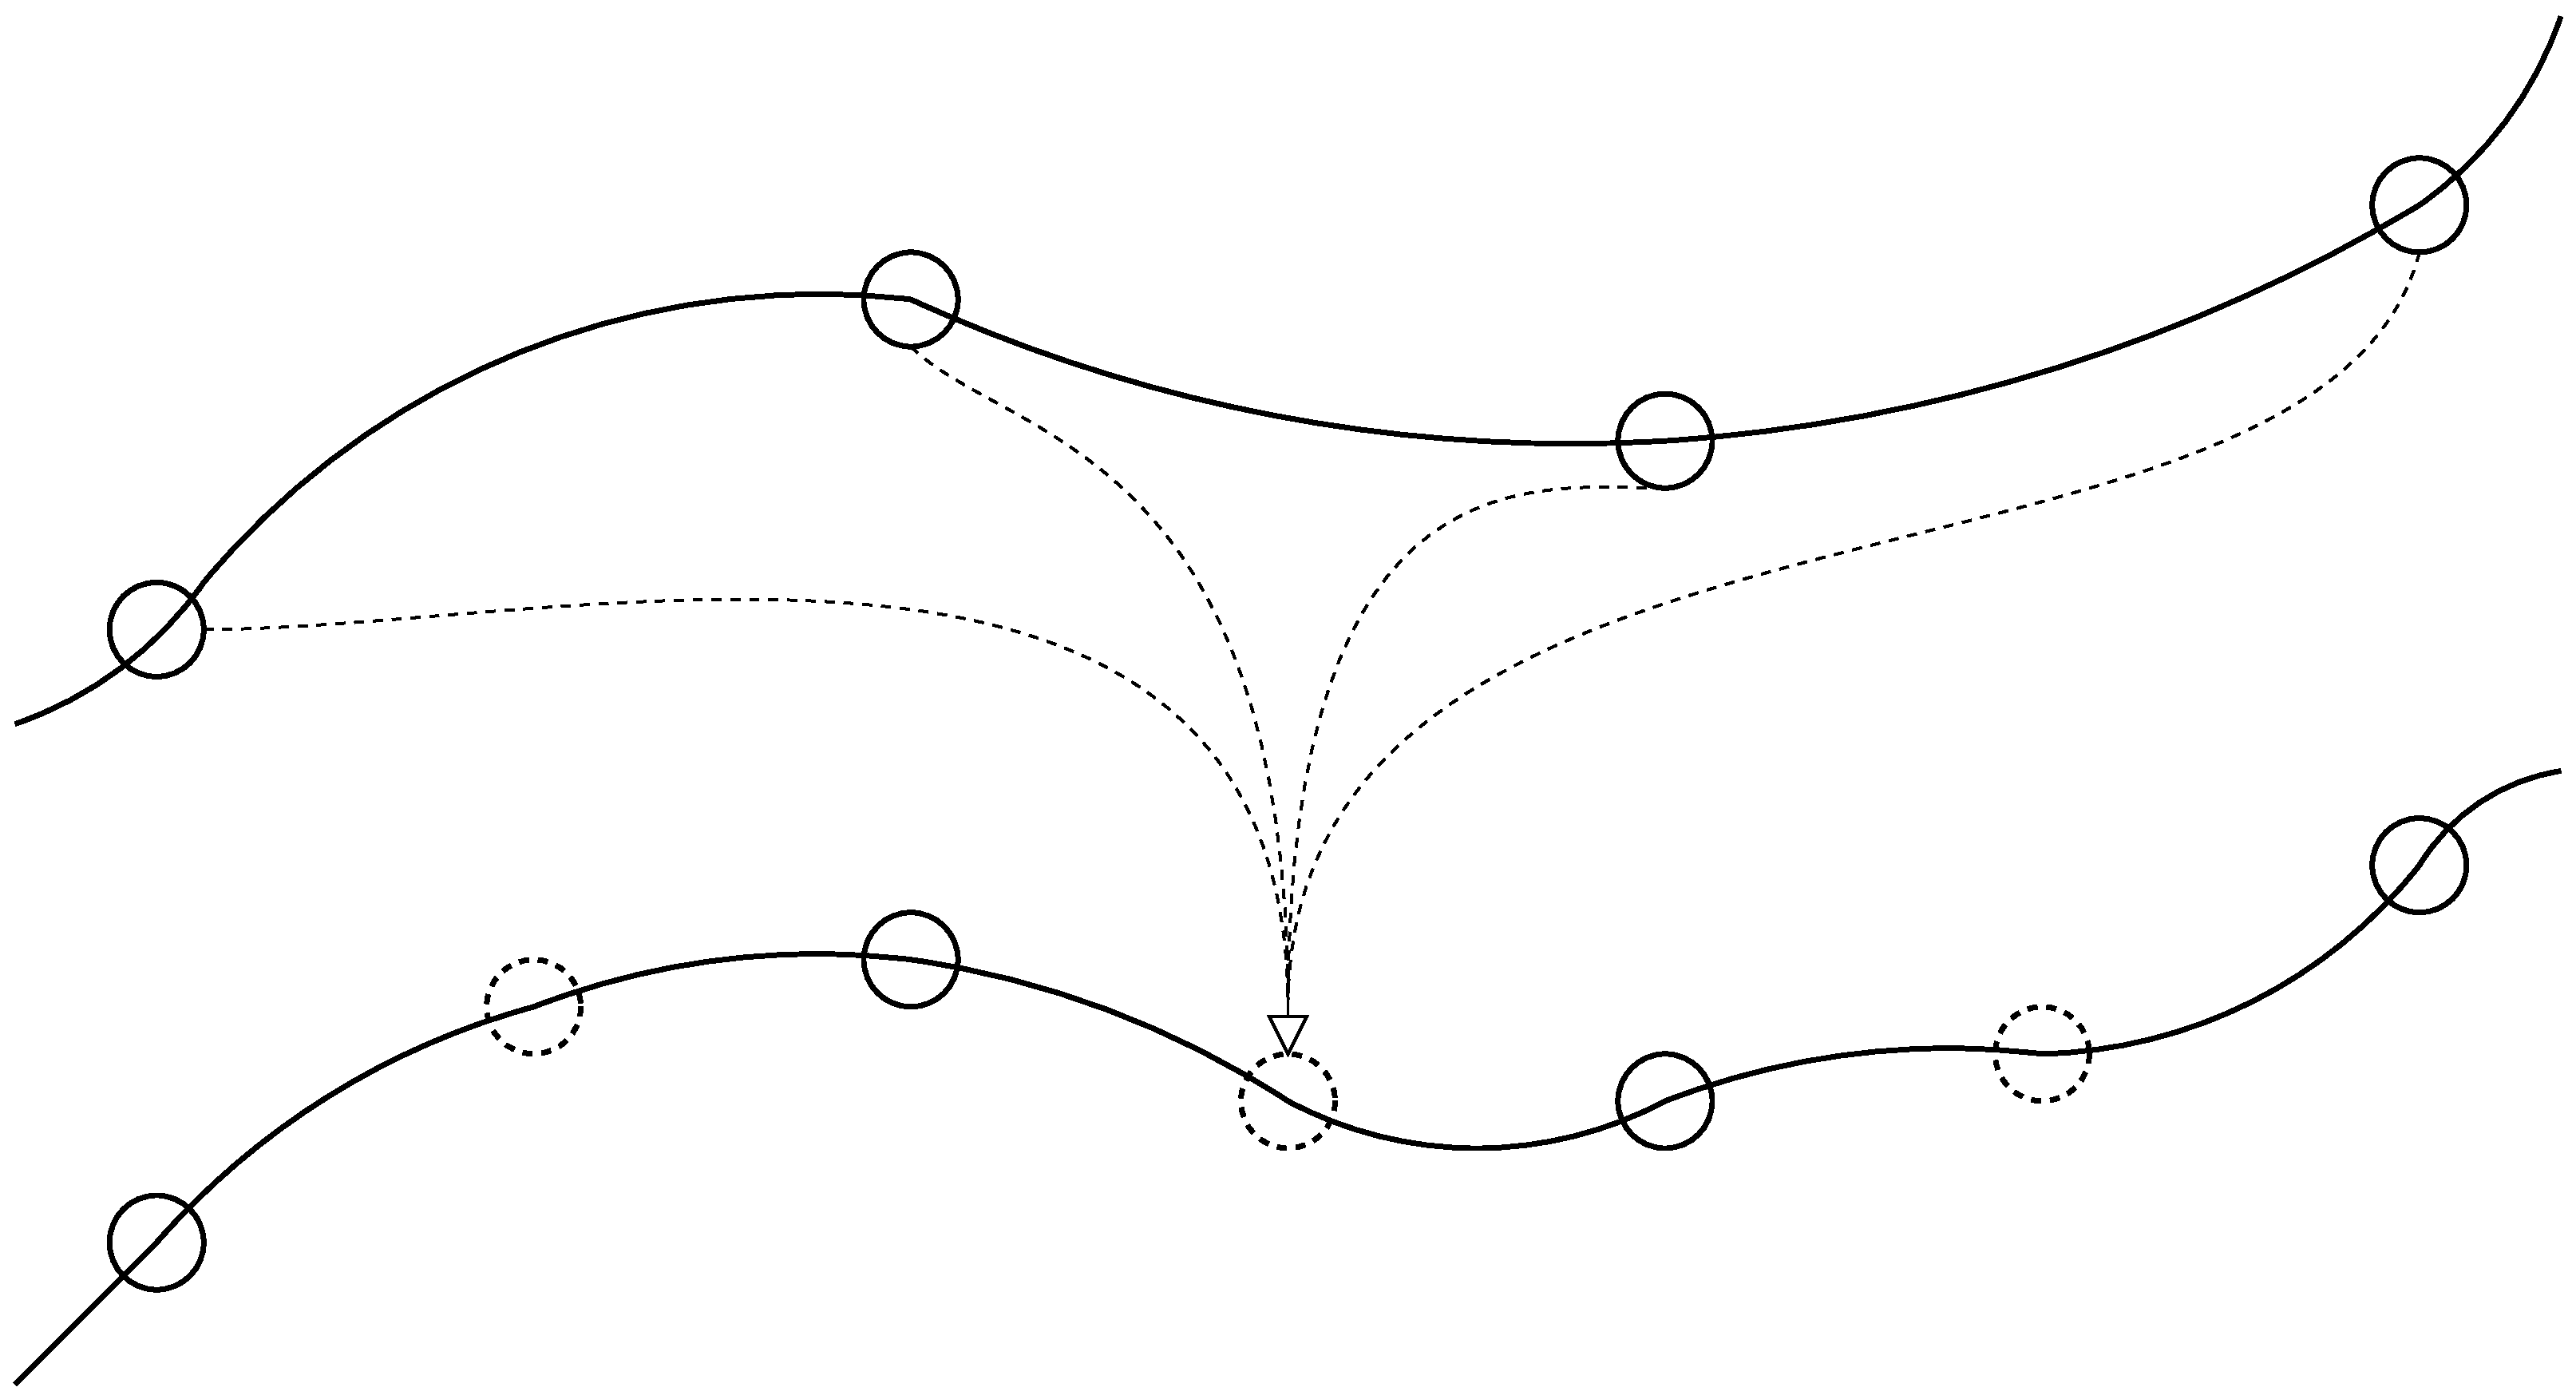
\includegraphics[  width=0.25\paperwidth,
 % keepaspectratio]{HRSdiagram}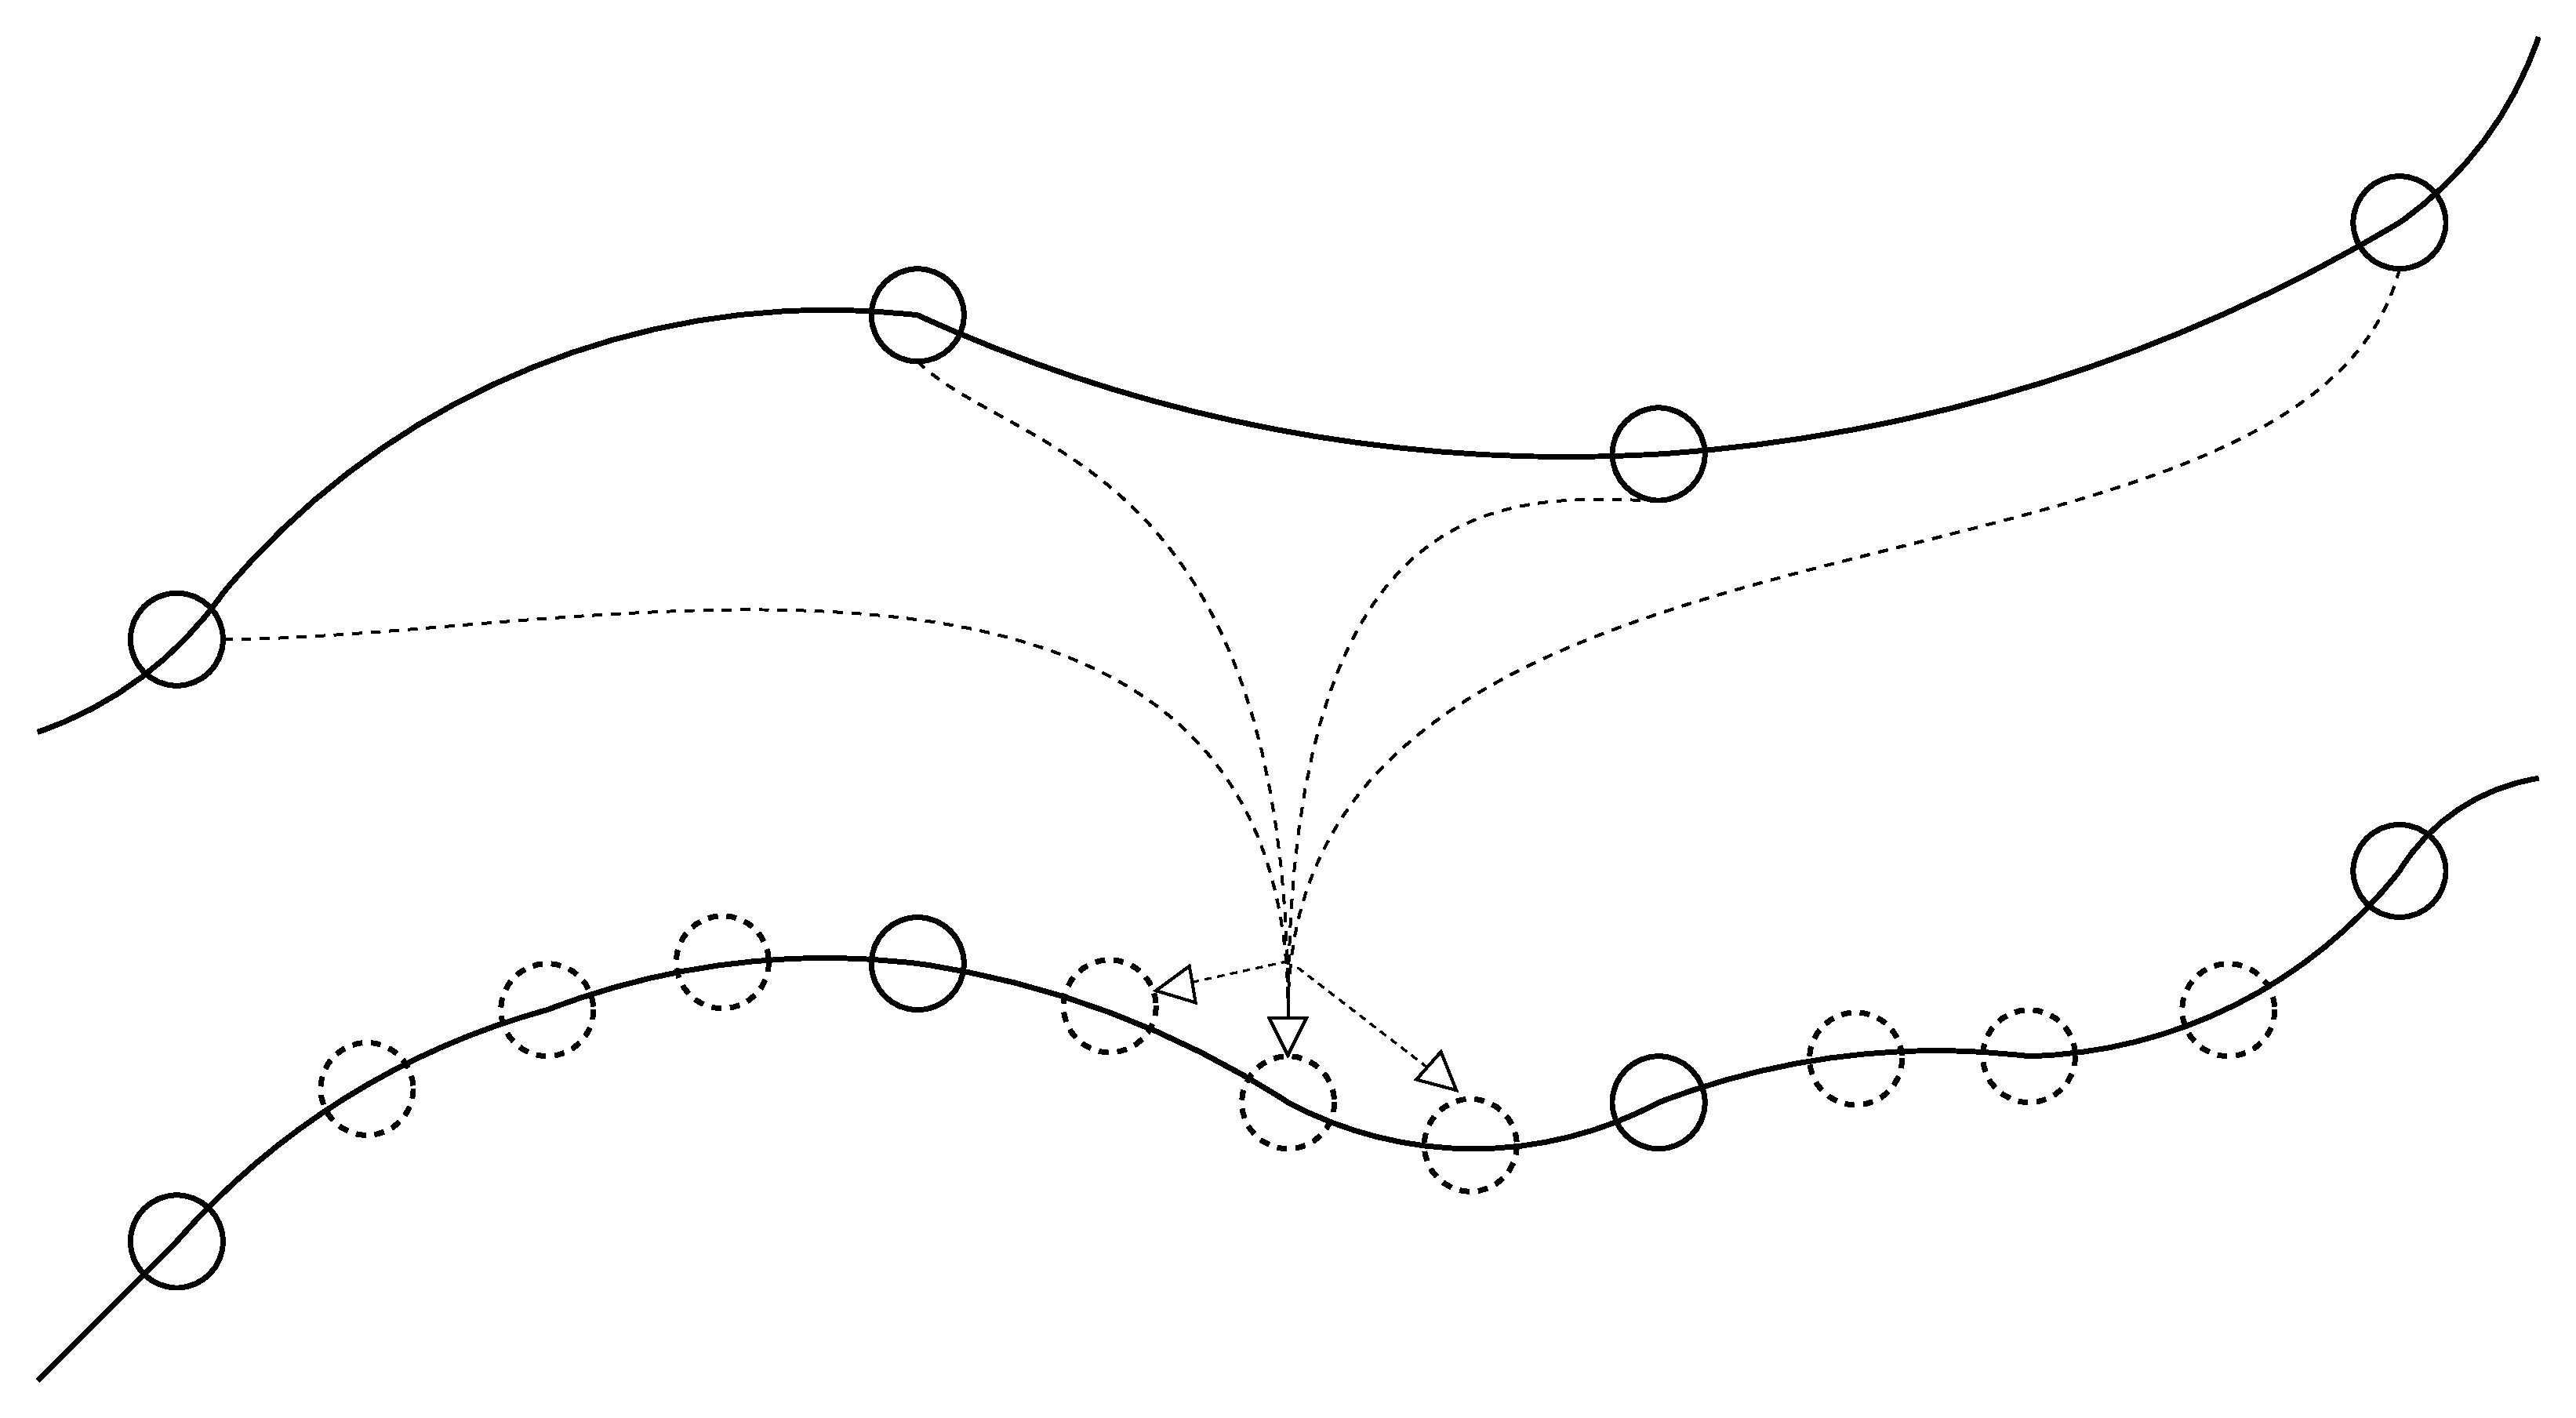
\includegraphics[  width=0.25\paperwidth]{HRSdiagram_tetradic}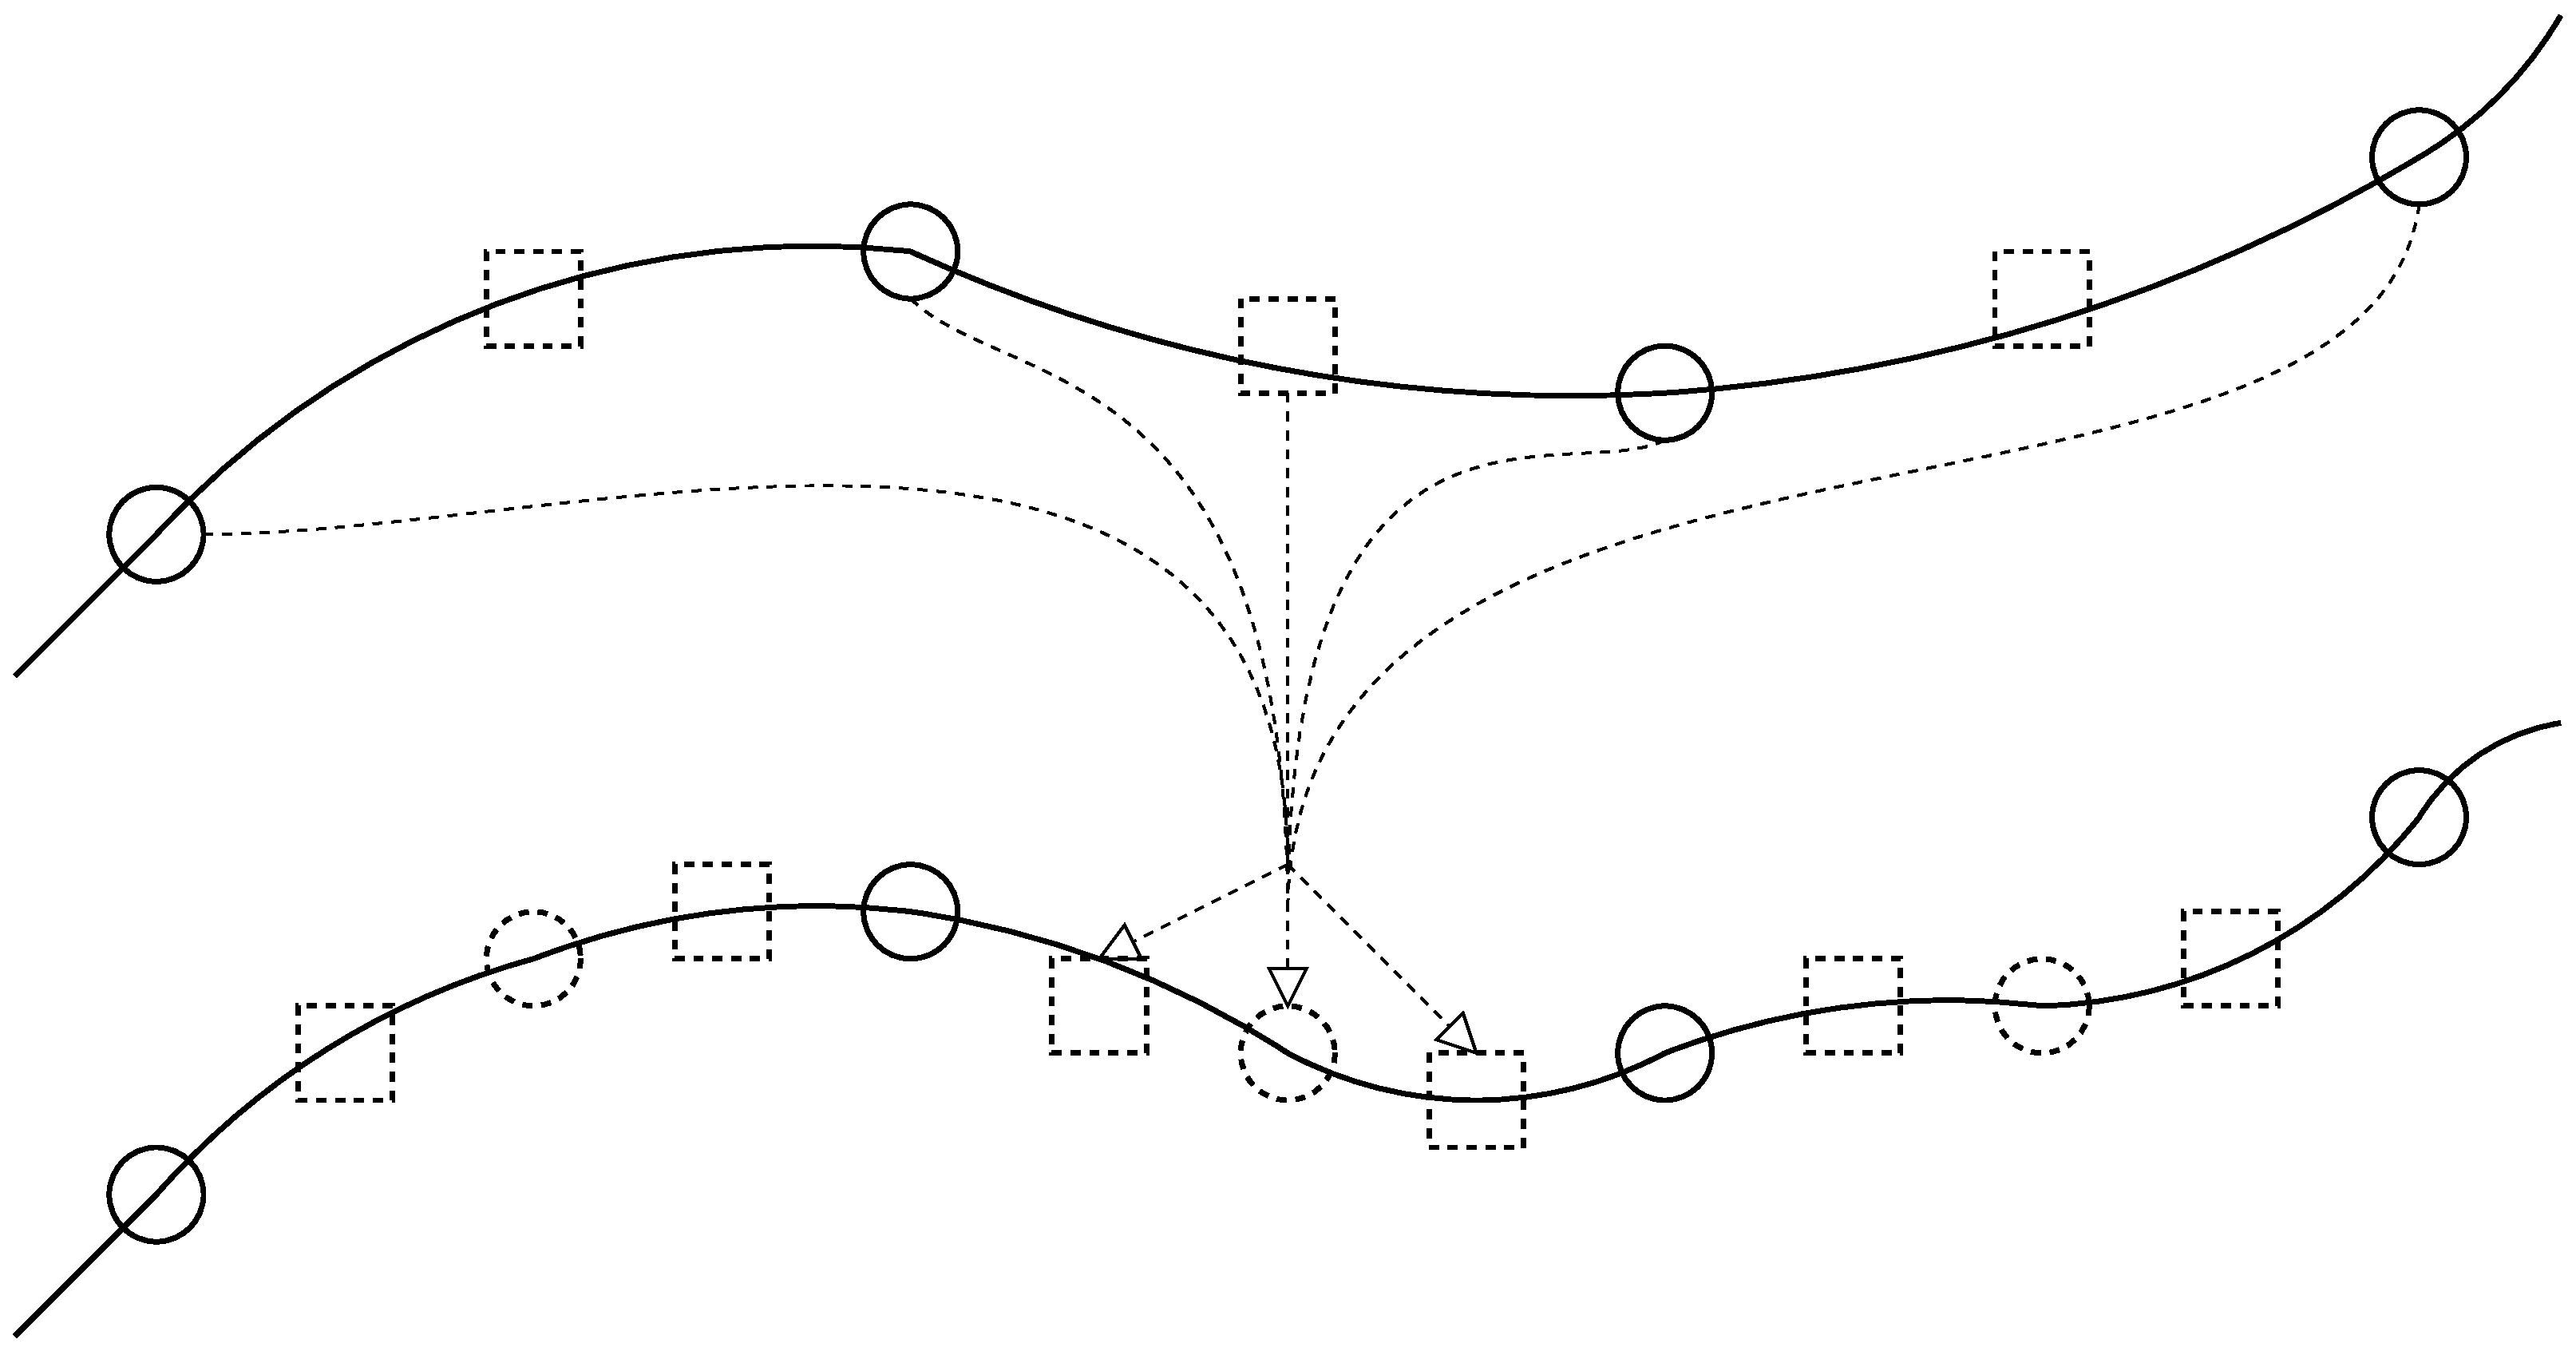
\includegraphics[  width=0.25\paperwidth,
  %keepaspectratio]{HRSdiagram2}\end{center}


%\figcaplong{Diagrams of 4-point subdivision schemes in the dyadic (left) and
%tetradic (center) cases, and HRS schemes (right). Arrows symbolize
%the interpolation process. The circles are data samples and, in the
%HRS diagram, the squares represent placeholders recording {}``guesses''. }

  
%************************ SECTION ************************
%************************ SECTION ************************
\sect{2. Subdivision Schemes}
%************************ SECTION ************************
%************************ SECTION ************************
  %% Insert text
  % $$ x = y. \en{}$$

  % \proclaim Theorem \pn{test}. Test.
  % \pf This is the proof. \eop

  
Let $b>1$ be an integer, a \dword{$b$-adic number} is of the form $x_{j,k}=k/b^{j}$
for some integers $k,j$. For a fixed $J$, given
some data $\left\{ y_{J,k}\right\} _{k\in \ZZ }$, we want a smooth
function $f$ such that $f\left(x_{J,k}\right)=y_{J,k}\, \forall k\in \ZZ $.
Starting with ($y_{J,k}$) and using the formula 
$$y_{j+1,l}=\sum _{k\in \ZZ }\gamma _{bk-l}y_{j,k}\en{basicsubdivision}$$
for some array $\gamma $, we get values $y_{j,k}$ for any $j>J$
and since $b$-adic numbers form a dense set in $\RR $, there is at
most one continuous function such that $f\left(x_{j,k}\right)=y_{j,k}$
for all $k\in \ZZ ,j>J$. 

A subdivision scheme is \dword{interpolatory} and satisfies $f\left(x_{J,k}\right)=y_{J,k}$
if $\gamma _{bk}=0\, \forall k\in \ZZ $ except for $\gamma _{0}=1$.
We say that a subdivision scheme is \dword{stationary} if the array
$\gamma $ is constant (does not depend on $j$). Because $\gamma $
does not depend explicitly on $l$ but rather on $bk-l$ the scheme
is \dword{translation invariant} or \dword{homogeneous}. A subdivision
scheme is a  \dword{$2N-$point scheme} if $\gamma _{l}=0$ for $|l|\geq Nb$. The \dword{fundamental
function} of an interpolatory $2N-$point $b$-adic scheme has initial
data $y_{0,0}=1$ and $y_{0,k}=0$ for all $k\neq 0$; it has a \dword{compact
support} of $[-(Nb-1)/(b-1),(Nb-1)/(b-1)]$ (or $[1-2N,2N-1]$ when
$b=2$). 

For $N=1,2,3,...$ there are corresponding interpolatory $2N-$point
\dword{Deslauriers-Dubuc subdivision schemes} built from the
midpoint evaluation of Lagrange polynomial of degree $2N-1$. For
$b=2$ (dyadic case), the 4-point Deslauriers-Dubuc scheme can
be defined with the array $\gamma ^{DD2}$ given by $\gamma _{0}^{DD2}=1,\, $$\gamma _{\pm 1}^{DD2}=-9/16,\, $$\gamma _{\pm 3}^{DD2}=-1/16$
with $\gamma _{k}^{DD2}=0$ otherwise; for $b=4$ (tetradic case),
the scheme is defined with the array $\gamma ^{DD4}$ given by $\gamma _{2k}^{DD4}=\gamma _{k}^{DD2}\, \forall k\in \ZZ ,\, $
$\gamma _{\pm 1}^{DD4}=105/128,\, $$\gamma _{\pm 3}^{DD4}=35/128,\, $$\gamma _{\pm 5}^{DD4}=-7/128,\, $$\gamma _{\pm 7}^{DD4}=-5/128,\, $with
$\gamma _{k}^{DD2}=0$ otherwise. 

Because 4-point Deslauriers-Dubuc schemes are derived from cubic
Lagrange polynomials, they reproduce cubic polynomials, that is, if
the initial data $y_{j,k}$ satisfies $y_{j,k}=p\left(x_{j,k}\right)\, \forall k\in \ZZ $
for some cubic polynomial $p$ then the interpolation function $f$
is this same cubic polynomial $f=p$. The two cases presented above
($\gamma ^{DD2}$ and $\gamma ^{DD4}$) converge to differentiable ($C^{1}$) interpolation
functions [\cit{Du},\cit{DeDu}].


%  Because we later borrow from these two subdivision schemes,
% we give explicit algorithms for both schemes.
% 
% \proclaim Algorithm~\pn{algo4pointdddyadicscheme}. (4-point Deslauriers-Dubuc Dyadic Scheme) For a given integer $j$,
% begin with some initial $y$ values $y_{j,k}\, k\in \ZZ $ over dyadic
% numbers $x_{j,k}=k/2^{j}$,
% \sm
% \ritem{1)} recopy data at $x_{j+1,2k}=x_{j,k}$: $y_{j+1,2k}=y_{j,k}\, \forall k\in \ZZ $;
% \sm
% \ritem{2)} interpolate midpoint value by the corresponding cubic Lagrange polynomial:
% $$
% y_{j+1,2k+1}=\frac{-y_{j,k-1}+9y_{j,k}+9y_{j,k+1}-y_{j,k+2}}{128}\, \forall k\in \ZZ ;$$
% \sm
% \ritem{3)} Repeat with $j\rightarrow j+1$ and using $y_{j+1}$ as initial data.
% \nopf
% 
% ~
% 
% \proclaim Algorithm~\pn{algo4pointtetradicscheme}. (4-point Deslauriers-Dubuc Tetradic Subdivision Scheme) For a given
% integer $j$, begin with some initial $y$ values $y_{j,k}\, k\in \ZZ $
% over tetradic numbers $x_{j,k}=k/4^{j}$
% \sm
% \ritem{1)} recopy data at $x_{j+1,4k}=x_{j,k}$: $y_{j+1,4k}=y_{j,k}\, \forall k\in \ZZ $;
% \sm
% \ritem{2)} interpolate quartile point values by the corresponding cubic Lagrange
% polynomial: $$
% y_{j+1,4k+1}=\frac{-7y_{j,k-1}+105y_{j,k}+35y_{j,k+1}-5y_{j,k+2}}{128};$$
 % $$
% y_{j+1,4k+2}=\frac{-y_{j,k-1}+9y_{j,k}+9y_{j,k+1}-y_{j,k+2}}{128};$$
% $$
% y_{j+1,4k+3}=\frac{-5y_{j,k-1}+35y_{j,k}+105y_{j,k+1}-7y_{j,k+2}}{128}\, \forall k\in \ZZ ;$$
% \sm
% \ritem{3)} Repeat with $j\rightarrow j+1$ and using $y_{j+1}$ as initial data.
% \nopf

  %************************ SECTION ************************  
%************************ SECTION ************************

%************************ SECTION ************************
%************************ SECTION ************************
  %% Insert text
  
  
  %****************subsection***********************
  \sect{3. High Resolution Subdivision Schemes}

We define stationary \dword{HRS schemes} by the equation
$$y_{j+1,l}=\sum _{m=1}^{M}\sum _{k\in \ZZ }\gamma _{Mbk+m-1-l}^{(m)}y_{j,Mk+m-1}\en{hrgeneral}$$
where $\gamma ^{(1)},...,\gamma ^{(M)}$ are constant arrays (independent
from $j$). They are \dword{$b$-adic scheme} because the number of nodes
increases by a factor of $b$ with each iteration. However, because
we have $M>1$ arrays $\gamma $, the scheme is said to be a HRS scheme.
It is an \dword{interpolatory scheme} if $y_{j+1,Mbk}=y_{j,Mk}$
and it is a \dword{$2N-$point scheme} if $\gamma _{l}^{(m)}=0$ for $|l|\geq MNb$
and $m=1,...,M$. 


For $b=M=2$ the general equation~\er{hrgeneral} becomes 
$$y_{j+1,l}=\sum _{k\in \ZZ }\gamma _{4k-l}^{(1)}y_{j,2k}+\gamma _{4k+1-l}^{(2)}y_{j,2k+1}.\en{N2highres}$$
%It is interpolatory if $y_{j+1,4k}=y_{j+1,2k}$ and $2N-$point if
%$\gamma _{l}^{(m)}=0$ for $|l|\geq 4N$ and $m=1,2$.  
A value $y_{j,k}$ is a \dword{stable value} if $y_{j,k}=y_{j+1,2k}$;
other nodes are said to be temporary or are referred to as \dword{placeholders}.
A HRS scheme on a dyadic grid is an \dword{interpolatory scheme} if all $y_{j,2k}$ values
on even nodes ($x_{j,2k}$) are stable so that $y_{j,2k}=y_{j+1,4k}\, \forall k\in \ZZ $.


%HRS schemes being multistep, given some data $\left\{ y_{j-1,k}\right\} _{k\in \ZZ }$ on the dyadic $x_{j-1,k}$
%grid, we apply a dyadic subdivision scheme as an initialization
%step. For 4-point HRS schemes, a sensible choice for the initialization step
%is the 4-point Deslauriers-Dubuc dyadic scheme (see lemma~\pr{lemmecubic})
%which copies the data at even nodes ($y_{j,2k}=y_{j-1,k}$) and insert
%new values ({}``guesses'') at odd nodes ($y_{j,2k+1}$ for $k\in \ZZ $).
%It should be noted that for the overall algorithm to be interpolatory,
%the initialization step must be interpolatory ($y_{j,bk}=y_{j-1,k}$).
%

%Assuming we used an interpolatory subdivision scheme as an initialization
%step, the following HRS algorithm is interpolatory.
%
%\proclaim Algorithm~\pn{4pointhrssalgo}. (4-point Dyadic HRS Schemes) The following
%iteration steps depend on $\alpha \in \RR $, a constant parameter.
%For a given integer $j$, begin with some initial $y$ values $y_{j,k}\, k\in \ZZ $
%over dyadic numbers $x_{j,k}=k/2^{j}$ where only the even nodes are
%interpolated ($y_{j,2k}$),
%\sm
%\ritem{1)} recopy stable data: $y_{j+1,4k}=y_{j,2k}\, \forall k\in \ZZ $ ;
%\sm
%\ritem{2)} Apply the 4-point Deslauriers-Dubuc tetradic scheme on even (stable)
%nodes: 
%$$y_{j+1,4k+1}=\frac{-7y_{j,2k-2}+105y_{j,2k}+35y_{j,2k+2}-5y_{j,2k+4}}{128};$$
%$$y_{j+1,4k+2}^{temporary}=\frac{-y_{j,2k-2}+9y_{j,2k}+9y_{j,2k+2}-y_{j,2k+4}}{128};$$
%$$y_{j+1,4k+3}=\frac{-5y_{j,2k-2}+35y_{j,2k}+105y_{j,2k+2}-7y_{j,2k+4}}{128}\, \forall k\in \ZZ ;$$
%\sm
%\ritem{3)} Update midpoint (which then becomes stable): $$y_{j+1,4k+2}=(1-\alpha )y_{j+1,4k+2}^{temporary}+\alpha y_{j,2k+1};$$
%\sm
%\ritem{4)} Repeat with $j\rightarrow j+1$ and using $y_{j+1}$ as initial data.
%\nopf
%
%This new algorithm is not a subdivision scheme in general and thus,
%we need a more general definition: stationary subdivision schemes
%(equation~\er{basicsubdivision}) can be generalized by the linear
%equation
%


%The interpolatory algorithm~\pr{4pointhrssalgo} amounts to choosing

For the rest of the paper, we will consider the schemes  $HRS_{\alpha }$ where
$\gamma ^{(1)}$ and $\gamma ^{(2)}$ are chosen to be $\gamma _{2k}^{(1)}=\gamma _{2k}^{DD4}+\alpha \left(\delta _{k,0}-\gamma _{k}^{DD2}\right)$,
$\gamma _{2k+1}^{(1)}=\gamma _{2k+1}^{DD4}\, \forall k\in \ZZ$, $\gamma _{0}^{(2)}=\alpha$, and $\gamma _{k}^{(2)}=0$ otherwise 
%$$\eqalignno{	&\enn{N2highres_1}\cr
%	   	\gamma _{0}^{(2)}=\alpha ,\,  & \gamma _{k}^{(2)}=0\, otherwise	&\enn{N2highres_2}}$$
%\begin{eqnarray}
%\gamma _{2k}^{(1)}=\gamma _{2k}^{DD4}+\alpha \left(\delta _{k,0}-\gamma _{k}^{DD2}\right),\,  & \gamma _{2k+1}^{(1)}=\gamma _{2k+1}^{DD4}\, \forall k\in \ZZ  & \label{N2highres_1}\\
%\gamma _{0}^{(2)}=\alpha ,\,  & \gamma _{k}^{(2)}=0\, otherwise & \label{N2highres_2}
%\end{eqnarray}
for some parameter $\alpha \in \RR $. Since $\gamma _{2k}^{DD4}=\gamma _{k}^{DD2}\, \forall k\in \ZZ $,
we can rewrite equation~\er{N2highres} for even and odd terms. Firstly,
setting $l=2s$ ($l$ even), we have 
$$ y_{j+1,2s}= \sum _{k\in \ZZ }  \left((1-\alpha )\gamma _{2k-s}^{DD2}+\alpha \delta _{2k,s}\right)y_{j,2k}+\delta _{2k+1,s+1}\alpha y_{j,2k+1}$$
%$$\eqalign{
%y_{j+1,2s} 	& =\sum _{k\in \ZZ }  \gamma _{4k-2s}^{(1)}y_{j,2k}+\gamma _{4k+1-2s}^{(2)}y_{j,2k+1} \cr
 %		& =\sum _{k\in \ZZ }  \left(\gamma _{4k-2s}^{DD4}-\alpha \gamma _{2k-s}^{DD2}+\alpha \delta _{4k,2s}\right)y_{j,2k}+\alpha \delta _{4k+1,s}y_{j,2k+1} \cr
 %		& =\sum _{k\in \ZZ }  \left((1-\alpha )\gamma _{2k-s}^{DD2}+\alpha \delta _{2k,s}\right)y_{j,2k}+\delta _{2k+1,s+1}\alpha y_{j,2k+1}
%}$$
%\begin{eqnarray*}
%y_{j+1,2s} & =\sum _{k\in \ZZ } & \gamma _{4k-2s}^{(1)}y_{j,2k}+\gamma _{4k+1-2s}^{(2)}y_{j,2k+1}\\
% & =\sum _{k\in \ZZ } & \left(\gamma _{4k-2s}^{DD4}-\alpha \gamma _{2k-s}^{DD2}+\alpha \delta _{4k,2s}\right)y_{j,2k}+\alpha \delta _{4k+1,s}y_{j,2k+1}\\
% & =\sum _{k\in \ZZ } & \left((1-\alpha )\gamma _{2k-s}^{DD2}+\alpha \delta _{2k,s}\right)y_{j,2k}+\delta _{2k+1,s+1}\alpha y_{j,2k+1}
%\end{eqnarray*}
so that when $s$ is even ($l=2s=4r$), we have the interpolatory
condition 
$$ y_{j+1,4r}=y_{j,2r}, \en{hrsinterpole}$$
otherwise, when $s$ is odd $(l=2s=4r+2)$
$$y_{j+1,4r+2}=\alpha y_{j,2r+1}+(1-\alpha )\sum _{k\in \ZZ }\gamma _{2k-2r-1}^{DD2}y_{j,2k}.\en{hrsricharson}$$
Secondly, if $l$ is odd ($l=2s+1$), we have
$$ y_{j+1,2s+1} = \sum _{k\in \ZZ }\gamma _{4k-2s-1}^{DD4}y_{j,2k}.   \en{hrswidguess}$$
%$$\eqalignno {
%y_{j+1,2s+1} & =  \sum _{k\in \ZZ }\gamma _{4k-2s-1}^{(1)}y_{j,2k}+\gamma _{4k-2s-1}^{(2)}y_{j,2k+1} &  \cr
%& =  \sum _{k\in \ZZ }\gamma _{4k-2s-1}^{DD4}y_{j,2k}. &  \enn{hrswidguess}\cr
%}$$
%\begin{eqnarray}
%y_{j+1,2s+1} & = & \sum _{k\in \ZZ }\gamma _{4k-2s-1}^{(1)}y_{j,2k}+\gamma _{4k-2s-1}^{(2)}y_{j,2k+1}\nonumber \\
 %& = & \sum _{k\in \ZZ }\gamma _{4k-2s-1}^{DD4}y_{j,2k}.\label{hrswidguess}
%\end{eqnarray}
Equations~\er{hrsinterpole}, \er{hrsricharson}, and \er{hrswidguess}
can be used to describe $HRS_{\alpha }$: while equation
\er{hrsinterpole} is the interpolatory condition, equation~\er{hrswidguess}
fills the placeholders with tetradic (coarse scale) interpolated values
whereas equation~\er{hrsricharson} combines the value stored in
the placeholder with the newly available interpolated value (fine
scale) given by the summation term which we recognize from the dyadic
Deslauriers-Dubuc interpolation. 

In the simplest case, $\alpha =0\Rightarrow \gamma ^{(2)}=0$ and equation~\er{N2highres} becomes
$y_{j+1,l}=\-\sum _{k\in \ZZ }\gamma _{4k-l}^{DD4}y_{j,2k}.$
This last equation discards odd nodes at each step: $y_{j+1,l}$ depends
only on even nodes ($y_{j,2k}$) and not at all on the odd nodes
($y_{j,2k+1}$). Hence, we have $y_{j+1,2l}=\sum _{k\in \ZZ }\gamma _{4k-2l}^{DD4}y_{j,2k}$
but because $\gamma _{2k}^{DD4}=\gamma _{k}^{DD2}$, this last equation
becomes $y_{j+1,2l}=\sum _{k\in \ZZ }\gamma _{2k-l}^{DD2}y_{j,2k}$ and if we define
$\widetilde{y}_{j,k}=y_{j,2k}$ we have that $HRS_{0 }$ is equivalent to the 4-point dyadic Deslauriers-Dubuc
subdivision scheme.  
%$$\widetilde{y}_{j+1,2l}=\sum _{k\in \ZZ }\gamma _{2k-l}^{DD2}\widetilde{y}_{j,2k}\en{DD2}$$
%which we recognize as the cubic Deslauriers-Dubuc scheme and we have
%proved the next proposition. 
%
%\proclaim Proposition~\pn{propDesDuequiv}. $HRS_{0 }$ is equivalent to the 4-point dyadic Deslauriers-Dubuc
%subdivision scheme.
%\nopf
%
%Thus we can say that the presented family of HRS schemes generalizes
%the dyadic Deslauriers-Dubuc scheme [\cit{Du},\cit{DeDu}].

%****************subsection***********************
\sect{4. Reproduced polynomials}
%****************subsection***********************

Assume that for some $j$, $y_{j,k}=p_{3}\left(x_{j,k}\right)\, \forall k\in \ZZ $
where $p_{3}$ is a cubic polynomial. Because 4-point Deslauriers-Dubuc
schemes reproduce cubic polynomials, we have $$
\sum _{k\in \ZZ }\gamma _{2k-2r-1}^{DD2}y_{j,2k}=y_{j,2r+1}=p_{3}\left(x_{j,2r+1}\right)$$
and thus equation~\er{hrsricharson} becomes $y_{j+1,4r+2}=p_{3}\left(x_{j,2r+1}\right)$
for any $\alpha \in \RR $. Similarly, equation~\er{hrswidguess}
implies $y_{j+1,2s+1}=p_{3}\left(x_{j+1,2s+1}\right)$. We conclude
that $y_{j+1,k}=p_{3}\left(x_{j+1,k}\right)\, \forall k\in \ZZ $ if
$y_{j,k}=p_{3}\left(x_{j,k}\right)\, \forall k\in \ZZ $ and thus $HRS_{\alpha }$ schemes
reproduce cubic polynomials. For practical implementations of a HRS
scheme, it is necessary to first apply a one-step subdivision scheme.
Let $\left\{ y_{j,k}\right\} _{k}$ be some initial data. As a first
step, we apply Deslauriers-Dubuc's equation
$$y_{j+1,l}=\sum _{k\in \ZZ }\gamma _{2k-l}^{DD2}y_{j,2k}\en{DD2_2}$$
 followed by $HRS_{\alpha }$ with $j+1$. This algorithm is as local as the corresponding
Deslauriers-Dubuc subdivision scheme in the sense that the fundamental
function has support $[-3,3]$. By induction
on $j$, we get the following
lemma.  
\proclaim Lemma~\pn{lemmecubic}. $HRS_{\alpha}$ schemes 
reproduce cubic polynomials and are interpolatory when using a one
step interpolatory 4-point dyadic Deslauriers-Dubuc interpolation
as initialization.
\nopf

We get a stronger result by choosing a specific $\alpha $.
We can write any quartic polynomial $p_{4}$ as $p_{4}(x)=a_{4}x^{4}+p_{3}(x)$
where $p_{3}$ is some cubic polynomial. Because of the Generalized
Rolle's theorem and because $\frac{p_{4}}{4!}=a_{4}$, given any 4 points $\xi _{1}$,$\xi _{2}$,$\xi _{3}$,
and $\xi _{4}$, the corresponding cubic polynomial $p_{Lagrange3}$
approximates $p_{4}$ with error 
$$p_{4}(x)-p_{Lagrange3}(x)  = a_{4}\left(x-\xi _{1}\right)\left(x-\xi _{2}\right)\left(x-\xi _{3}\right)\left(x-\xi _{4}\right) \en{rolleeq}$$
for some $\xi $. In other words, the error depends only on $a_{4}$
and the geometry of the sample points $\xi _{i}$ with respect to
$x$. This makes the task of canceling out the errors convenient as we shall see.

Suppose that for some $j$, $y_{j,2k}=p_{4}\left(x_{j,2k}\right)$
and $y_{j-1,k}=p_{4}\left(x_{j-1,k}\right)\, \forall k\in \ZZ $. We
can write $y_{j+1,4r+2}$ for any $r\in \ZZ $ in terms of this initial
data ($y_{j}$ and $y_{j-1}$) by substituting equation~\er{hrswidguess}
into~\er{hrsricharson} to get 
$$\eqalignno{
y_{j+1,4r+2} & =  \alpha y_{j,2r+1}+(1-\alpha )\sum _{k\in \ZZ }\gamma _{2k-2r-1}^{DD2}y_{j,2k} & \cr
 & =  \alpha \sum _{k\in \ZZ }\gamma _{4k-2r-1}^{DD4}y_{j-1,2k}+(1-\alpha )\sum _{k\in \ZZ }\gamma _{2k-2r-1}^{DD2}y_{j,2k}.&\enn{upcomingrichardson}}$$
We want to show that $y_{j+1,4r+2}=p_{4}\left(x_{j,2r+1}\right)$
for some $\alpha \in \RR $ and so we substitute $y_{j,2k}=p_{4}\left(x_{j,2k}\right)$
and $y_{j-1,k}=p_{4}\left(x_{j-1,k}\right)$ into the two sums of
this last equation. We compute both sums in equation~\er{upcomingrichardson} explicitly using equation~\er{rolleeq} (Rolle's):
$$
\sum _{k\in \ZZ }\gamma _{4k-2r-1}^{DD4}y_{j-1,2k} =  p_{4}\left(x_{j,2r+1}\right)-\frac{105a_{4}}{2^{4j}}  \en{105sur16}$$
%$$\eqalignno {
%\sum _{k\in \ZZ }\gamma _{4k-2r-1}^{DD4}y_{j-1,2k} & =  p_{3}\left(x_{j,2r+1}\right)+a_{4}\sum _{k\in \ZZ }\gamma _{4k-2r-1}^{DD4} \left(x_{j,4k}\right)^{4}& \cr
%  = & p_{4}\left(x_{j,2r+1}\right)-\frac{105a_{4}}{2^{4j}} & \enn{105sur16}
%}$$
 and similarly $\sum _{k\in \ZZ }\gamma _{2k-2r-1}^{DD2}y_{j,2k} = p_{4}\left(x_{j,2r+1}\right)-\frac{9a_{4}}{2^{4j}}$.
 %$$\eqalign {
%\sum _{k\in \ZZ }\gamma _{2k-2r-1}^{DD2}y_{j,2k} & =  p_{3}\left(x_{j,2r+1}\right)+a_{4}\sum _{k\in \ZZ }\gamma _{2k-2r-1}^{DD2} \left(x_{j,2k}\right)^{4}\cr
% & =  p_{4}\left(x_{j,2r+1}\right)-\frac{9a_{4}}{2^{4j}}.
%}$$
Hence, setting $\alpha =-3/32$ in equation~\er{upcomingrichardson},
we get $$
y_{j+1,4r+2}=p_{4}\left(x_{j,2r+1}\right)-\frac{105\alpha +9(1-\alpha )}{2^{4j}}a_{4}=p_{4}\left(x_{j+1,4r+2}\right)$$
%since for $\alpha =-3/32$, $105\alpha +9(1-\alpha )=0$. 
Therefore, $HRS_{-3/32}$ reproduces quartic polynomials once the data has been properly
initialized. While there are no 4-point subdivision scheme capable
of interpolating $y_{j-1,k}=p_{4}\left(x_{j,k}\right)$ into $y_{j,2k+1}=p_{4}\left(x_{j,2k+1}\right)-\frac{105a_{4}}{16\times 2^{4j}}$
and $y_{j,2k}=p_{4}\left(x_{j,2k}\right)$ for all $k\in \ZZ $, there
exist 5-point subdivision schemes such as the subdivision scheme
described by the next algorithm.

\proclaim Algorithm~\pn{5pointalgo}. (5-point {}``Initialization'' Subdivision
Scheme) For a given integer $j$, begin with some initial $y$ values
$y_{j,k}\, k\in \ZZ $ over dyadic numbers $x_{j,k}=k/2^{j}$,
\sm
\ritem{1)} recopy data at $x_{j+1,2k}=x_{j,k}$: $y_{j+1,2k}=y_{j,k}\, \forall k\in \ZZ $;
\sm
\ritem{2)} extrapolate $y_{j,k+4}$ using $y_{j,k-2},y_{j,k-1},y_{j,k},y_{j,k+1},y_{j,k+2}$
by the formula 
$\gamma _{j,k}=5y_{j,k-2}-24y_{j,k-1}+45y_{j,k}-40y_{j,k+1}+15y_{j,k+1}$, $\forall k\in \ZZ ;$
\sm
\ritem{3)} interpolate midpoint value using the tetradic Deslauriers-Dubuc formula
$
y_{j+1,2k+1}=\frac{-7y_{j,k-2}+105y_{j,k}+35y_{j,k+2}-5\gamma _{j,k}}{128}$ $\forall k\in \ZZ$.
\nopf

To see that algorithm~\pr{5pointalgo} properly initializes the placeholders,
observe that if we assume $y_{J,k}=p_{4}\left(x_{J,k}\right)$,
then we only need to check that $y_{J+1,2k+1}=p_{4}\left(x_{J+1,2k+1}\right)-\frac{105a_{4}}{16\times 2^{4(J+1)}}$.
However, if $y_{J,k}=p_{4}\left(x_{J,k}\right)$ is satisfied, then
$\gamma _{J,k}=p_{4}\left(x_{J,k+4}\right)$ since it
can be derived by finding the quartic polynomial $p_{J,k}$ satisfying
$p_{J,k}\left(x_{j,l}\right)=y_{J,l}$ for $l=k-2,...,k+2$ and setting
$\gamma _{J,k}=p_{J,k}\left(x_{J,k+4}\right)$. Hence, by equation
\er{105sur16}, we have the following lemma.

\proclaim Lemma~\pn{5pointlemma}. Algorithm~\pr{5pointalgo} describes a 5-point dyadic subdivision
scheme such that with $y_{j-1,k}=p_{4}\left(x_{j-1,k}\right)$ where
$p_{4}(x)=a_{4}x^{4}+a_{3}x^{3}+a_{2}x^{2}+a_{1}x+a_{0}$ is a quartic
polynomial, $y_{j,2k+1}=p_{4}\left(x_{j,2k+1}\right)-\frac{105a_{4}}{16\times 2^{4j}}$
and $y_{j,2k}=p_{4}\left(x_{j,2k}\right)$ for all $k\in \ZZ $.
\nopf

Then, because we have a proper initialization scheme, we can reproduce
quartic polynomials as the next proposition states.

\proclaim Proposition~\pn{prop4}. $HRS_{-3/32}$ with algorithm~\pr{5pointalgo}
as an initialization step, reproduce quartic polynomials.
\nopf

%This result is significant because it is not possible for 4-point
%subdivision schemes to reproduce quartic polynomials. Even if we include
%non-interpolatory subdivision schemes, for a given $k\in \ZZ $, $y_{j+1,2k+1}$
%cannot be computed solely from the neighboring values $y_{j,k-1}$,
%$y_{j,k}$,$y_{j,k+1}$, and $y_{j,k+1}$ while reproducing quartic
%polynomials. Indeed, let $P_{4}(x)=x(x-1)(x-2)(x-3)$ and consider
%$y_{0,k}=P_{4}(k)$. All 4-point subdivision schemes interpolate
%$y_{1,3}=0\neq P_{4}\left(\frac{3}{2}\right)=\frac{9}{16}$. Thus,
%we see that
%
Only subdivision schemes using at least 5 points can interpolate
quartic polynomials and the support
of the fundamental function is at least of \eword{size 8} whereas the
algorithm described by proposition \pr{prop4} ($HRS_{-3/32}$) leads to fundamental functions having compact support of  
\eword{size 7} taking into account the 5-point initialization scheme. 
%For example,
%consider schemes of the form $y_{j+1,l}=\sum _{k=-2}^{2}\tau _{2k-l}y_{j,k}$
%with $\tau _{-5}=\frac{3}{128},$$\tau _{-3}=\frac{-5}{32},$$\tau _{-1}=\frac{45}{64}$,$\tau _{1}=\frac{15}{32}$,$\tau _{3}=\frac{-5}{128}$
%and $\tau _{0}=1$, $\tau _{k}=0$ otherwise which has support $[-3,5]$.
%On the other hand, applying the algorithm described by proposition

%Therefore, we have a new quartic interpolation scheme more local than
%5-point quartic dyadic subdivision schemes. Such good local properties
%are possible because in $HRS_{\alpha}$, the placeholders
%are only used to predict upcoming interpolations except maybe during
%the initialization.
%

\sect{5. Sufficient conditions for regularity}

Given that $HRS_{0 }$ is equivalent
to the Deslauriers-Dubuc subdivision which is $C^{1}$, it is reasonable
to expect $HRS_{\alpha }$ to be $C^{1}$ for some range of $\alpha $
values. Moreover, motivated by proposition~\pr{prop4}, we need to
show that this range of values includes $\alpha =-3/32$. At this point,
it is convenient to rewrite equation~\er{N2highres} in terms of (trigonometric) \dword{Laurent polynomials}.
Given some data $y_{j,k}$, define $P^{j}(z)=\sum _{k\in \ZZ }y_{j,k}z^{k}$.
If $P_{2}(z)=\sum _{k\in \ZZ }\gamma _{k}^{DD2}z^{k}$, then the equation
of the 4-point dyadic Deslauriers-Dubuc scheme (equation~\er{DD2_2}),
can be rewritten $P^{j+1}(z)=P_{2}(z)P^{j}(z^{2})$. Similarly, if
$P_{4}(z)=\sum _{k\in \ZZ }\gamma _{k}^{DD4}z^{k}$, then the tetradic
subdivision scheme is given by $P^{j+1}(z)=P_{4}(z)P^{j}(z^{2})$.
We can rewrite the general equation for $b-$ adic HRS schemes as 
$$P^{j+1}(z)=\sum _{i=1}^{M}\Gamma _{i}(z)P^{j}\left(e^{2\pi i/b}z^{b}\right)$$
where the $\Gamma _{i}$ must be Laurent polynomials. For
dyadic HRS schemes ($b=2$), this equation becomes 
$$P^{j+1}(z)=\Gamma _{1}(z)P^{j}\left(z^{2}\right)+\Gamma _{2}(z)P^{j}\left(-z^{2}\right).\en{gammas}$$
The $HRS_{\alpha }$ \dword{symbols} are 
$$\eqalign{
\Gamma _{1}(z) & =  \Gamma _{2}(z)+\alpha \cr
\Gamma _{2}(z) & =  \frac{P_{4}\left(z\right)-P_{4}\left(-z\right)}{4}+(1-\alpha )\frac{P_{4}\left(z\right)+P_{4}\left(-z\right)}{4}.
}$$
%When $\alpha =0$ (Deslauriers-Dubuc case), $\Gamma _{1}(z)=\Gamma _{2}(z)=\frac{P_{4}\left(z\right)}{2}$
%and equation~\er{N2highres} becomes$$
%P^{j+1}(z)=P_{4}\left(z\right)\left(\frac{P^{j}\left(z^{2}\right)+P^{j}\left(-z^{2}\right)}{2}\right).$$
%Averaging $P^{j+1}(z)$ and $P^{j+1}(-z)$ 
%$$\eqalign {
%\frac{P^{j+1}(z)+P^{j+1}(-z)}{2} & =  \left(\frac{P_{4}\left(z\right)-P_{4}\left(-z\right)}{2}\right)\left(\frac{P^{j}\left(z^{2}\right)+P^{j}\left(-z^{2}\right)}{2}\right)\cr
% & =  P_{2}\left(z^{2}\right)\left(\frac{P^{j}\left(z^{2}\right)+P^{j}\left(-z^{2}\right)}{2}\right).
%}$$
%we rediscover that when $\alpha =0$ the HRS scheme becomes the dyadic
%Deslauriers-Dubuc scheme (proposition~\pr{propDesDuequiv}).
%
Following Dyn \cite{Dyn}, we want to find corresponding schemes for
the (forward) finite differences. Let $dx_{j}=1/2^{j}$ and write
$$
D_{j,k}=\frac{dy_{j,k}}{dx_{j}}=2^{j}\left(y_{j,k+1}-y_{j,k}\right),$$
and define higher order finite differences recursively 
%$$D_{j,k}^{n}=d^{(n)}y_{j,k}/\left(dx_{j}\right)^{n}=d\left(d^{(n-1)}y_{j,k}\right)/\left(dx_{j}\right)^{n}=2^{jn} d^{(n)}y_{j,k}.$$
$$D_{j,k}^{n}=d^{(n)}y_{j,k}/\left(dx_{j}\right)^{n}=2^{jn} d^{(n)}y_{j,k}.$$
 Because $\sum _{k\in \ZZ }2^{j}\left(y_{j,k+1}-y_{j,k}\right)z^{k} =  \sum _{k\in \ZZ }2^{j}y_{j,k}z^{k-1}-\sum _{k\in \ZZ }2^{j}y_{j,k}z^{k}$,
we have  
 % 
% Note that $D_{j,k}=D_{j,k}^{1}$. Let $H_{1}^{j}$ be the symbol
%for $D_{j,k}^{1}$, then $$\eqalign{
%H_{1}^{j}(z) & =  \sum _{k\in \ZZ }2^{j}\left(y_{j,k+1}-y_{j,k}\right)z^{k}\cr
% & =  \sum _{k\in \ZZ }2^{j}y_{j,k}z^{k-1}-\sum _{k\in \ZZ }2^{j}y_{j,k}z^{k}\cr
% & =  2^{j}(1/z-1)P^{j}(z)=2^{j}(1-z)P^{j}(z)/z,
%}$$
% and thus $P^{j}\left(z^{2}\right)=z^{2}2^{j}H_{1}^{j}\left(z^{2}\right)/(1-z^{2})$,
%$P^{j}\left(-z^{2}\right)=-z^{2}2^{j}H_{1}^{j}\left(-z^{2}\right)/(1+z^{2})$,
%and $P^{j+1}(z)=z2^{j+1}H_{1}^{j+1}(z)/(1-z)$. Substituting these
%three equations into equation~\er{gammas} gives
%$$H_{1}^{j+1}(z)=\frac{2z(1-z)}{(1-z^{2})}\Gamma _{1}(z)H_{1}^{j}\left(z^{2}\right)-\frac{2z(1-z)}{(1+z^{2})}\Gamma _{2}(z)H_{1}^{j}\left(-z^{2}\right).\en{notsogen}$$
% Similarly, the higher order finite differences are given by
 $$
H_{n}^{j}(z)=\frac{2(1-z)}{z}H_{n-1}^{j}(z)=\left(\frac{2(1-z)}{z}\right)^{n}P^{j}(z)$$
where $H_{0}(z)=P(z)$ and they can be computed by 
$$\eqalignno{
H_{n}^{j+1}(z)& =\left(\frac{2z}{1+z}\right)^{n}\Gamma _{1}(z)H_{n}^{j}\left(z^{2}\right) & \cr
		& +\left(\frac{-2z(1-z)}{1+z^{2}}\right)^{n}\Gamma _{2}(z)H_{n}^{j}\left(-z^{2}\right).&\enn{genh}
}$$
$H_{n}$ is the symbol of a HRS scheme if $n=1,2,3,4$ because $\Gamma _{1}(z)/(1+z)^{n}$
and $\Gamma _{2}(z)/(1+z^{2})^{n}$ are Laurent polynomials

%$dH_{n}^{j}$ as 
%the symbol of 
%$$dD_{j,k}^{n-1}=d\left(\frac{d^{(n-1)}y_{j,k}}{\left(dx_{j}\right)^{n-1}}\right)=\frac{d^{n}y_{j,k}}{\left(dx_{j}\right)^{n-1}}=\frac{D_{j,k}^{n}}{2^{j}}$$
%$$dD_{j,k}^{n-1}=\frac{d^{n}y_{j,k}}{\left(dx_{j}\right)^{n-1}}=\frac{D_{j,k}^{n}}{2^{j}}$$
% or
 We define $dH_{n}^{j}(z)=H_{n+1}^{j}(z)/2^{j}$ as symbols of $dD_{j,k}^{n-1}=d\frac{dy_{j,k}}{dx_{j}}$
 and since $dH_{n}^{j}(z)=H_{n+1}^{j}(z)/2^{j}$, $dH_{n-1}$ is
the symbol of a HRS scheme for $n=1,2,3,4$. Using results from Dyn \cite{Dyn}, we have the following theorem.
% $$dH_{n-1}^{j}(z)=\frac{(1-z)}{z}H_{n-1}^{j}(z)=\frac{2^{j(n-1)}(1-z)^{n}}{z^{n}}P^{j}(z).\en{dHdef}$$
%Replacing $H_{n-1}$ by $dH_{n-1}$ in equation~\er{genh}, we find

%
%

%$$\eqalignno{
%dH_{n-1}^{j+1}(z) & =\frac{1}{2} \left(\frac{2z}{1+z}\right)^{n}\Gamma _{1}(z)dH_{n-1}^{j}\left(z^{2}\right)  & \cr
%& +\frac{1}{2}\left(\frac{-2z(1-z)}{1+z^{2}}\right)^{n}\Gamma _{2}(z)dH_{n-1}^{j}\left(-z^{2}\right)\ . & \enn{dH}}$$
%And because $dH_{n}^{j}(z)=H_{n+1}^{j}(z)/2^{j}$, $dH_{n-1}$ is
%the symbol of a HRS scheme for $n=1,2,3,4$. 



\proclaim Theorem~\pn{DynTheorem}. (Dyn-Levin) Given trigonometric polynomials $\Gamma _{1}(z)$
and $\Gamma _{2}(z)$, the HRS scheme defined by $
P^{j+1}(z)=\Gamma _{1}(z)P^{j}\left(z^{2}\right)+\Gamma _{2}(z)P^{j}\left(-z^{2}\right)$
 is $C^{n}$ if the symbol corresponding to finite differences of
order $n+1$, $dH_{n}^{j}(z)=\frac{2^{jn}(1-z)^{n+1}}{z^{n+1}}P^{j}(z)$
 is the symbol of a HRS scheme converging uniformly to zero for all
bounded initial data.

\pf
See the proof of theorem 3.4 in \cite{Dyn} or section 4.2 in \cite{DynLevin}
as it applies to HRS schemes. The key point being that for an iterative
interpolation scheme (even a nonstationary one) to be $C^{n}$, it
is sufficient for the finite differences $d^{n+1}y_{j,k}/\left(dx_{j}\right)^{n}$
to converge uniformly to zero. 
\eop


In general, given $y_{j+1,l}=\sum _{k\in \ZZ }\gamma _{2k-l}y_{j,k}$,
a sufficient condition for $y_{j,k}\rightarrow 0$ uniformly as $j\rightarrow \infty $
is that $\lambda =\max _{l=0,1}\left\{ \sum _{k\in \ZZ }\left|\gamma _{2k-l}\right|\right\} <1$.
%,
%indeed, if $M_{j}=\sup \left\{ \left|y_{j,k}\right|:k\in \ZZ \right\} $
%then $M_{j+1}\leq \max _{l=0,1}\left\{ \sum _{k\in \ZZ }\left|\gamma _{2k-l}\right|\right\} M_{j}$
%because $y_{j+1,2l}=\sum _{k\in \ZZ }\gamma _{2k-2l}y_{j,k}$ and $y_{j+1,2l+1}=\sum _{k\in \ZZ }\gamma _{2k-2l-1}y_{j,k}$.
For a HRS scheme given by $y_{j+1,l}=\sum _{k\in \ZZ }\gamma _{4k-l}^{(1)}y_{j,2k}+\gamma _{4k+1-l}^{(2)}y_{j,2k+1}$,
%,  $y_{j+1,2l}=\sum _{k\in \ZZ }\gamma _{4k-2l}^{(1)}y_{j,2k}+\gamma _{4k+1-2l}^{(2)}y_{j,2k+1}$
%and $y_{j+1,2l+1}=\sum _{k\in \ZZ }\gamma _{4k-2l-1}^{(1)}y_{j,2k}+\gamma _{4k-2l}^{(2)}y_{j,2k+1}$.
$\lambda _{HR}=\max _{l=0,1}\left\{ \sum _{k\in \ZZ }\left|\gamma _{2k-l}^{(1)}\right|+\left|\gamma _{2k+1-l}^{(2)}\right|\right\} $
implies $M_{j+1}\leq \lambda _{HR} M_{j}$  where $M_{j}=\sup \left\{ \left|y_{j,k}\right|:k\in \ZZ \right\} $. 
To write this statement in symbols, 
define $\left\Vert Q(z)\right\Vert _{sup}=\sup _{k}\left\{ \left|q_{k}\right|\right\} $
and $\left\Vert Q(z)\right\Vert _{\Sigma }=\max \left\{ \sum _{k}\left|q_{k}\right|\right\} $ where $Q(z)=\sum _{k}q_{k}z^{k}$.
Now, if $P^{j+1}(z)=\tilde \Gamma _{1}(z)P^{j}\left(z^{2}\right)+\tilde \Gamma _{2}(z)P^{j}\left(-z^{2}\right)$ and
$$\lambda _{HR}= \max \left\{ \lambda _{1},\lambda _{2}\right\} \en{lemmaenough} $$ 
where $2 \lambda _{1/2} = \left\Vert \tilde \Gamma _{1}(z) \pm \tilde \Gamma _{1}(-z)+\tilde \Gamma _{2}(z) \mp \tilde \Gamma _{2}(-z)\right\Vert _{\Sigma }$,
%$$\eqalign{
%\lambda _{1} &= \left\Vert \frac{\Lambda _{1}(z)+\Lambda _{1}(-z)+\Phi _{2}(z)-\Lambda _{2}(-z)}{2}\right\Vert _{\sum } \cr
%\lambda _{2} &= \left\Vert \frac{\Lambda _{1}(z)-\Lambda _{1}(-z)+\Phi _{2}(z)+\Lambda _{2}(-z)}{2}\right\Vert _{\sum } 
%}$$
then $$\left\Vert P^{j+1}(z)\right\Vert _{sup}\leq \lambda _{HR}\left\Vert P^{j}(z)\right\Vert _{sup}.$$

\proclaim Lemma~\pn{enoughlemma}. A HRS scheme given by the symbol equation $P^{j+1}(z)=\tilde \Gamma _{1}(z)P^{j}\left(z^{2}\right)+\tilde \Gamma _{2}(z)P^{j}\left(-z^{2}\right)$
converges uniformly to zero for all bounded initial values if $\lambda _{HR}<1$
where $\lambda _{HR}$ is as in equation~\er{lemmaenough}.
\nopf

We are now ready to prove the following theorem which shows that $HRS_{\alpha }$ are smooth for
$\alpha $ near 0 (see Fig.~\fr{Figdifffund}).% (see Fig.~\fr{Figdifffund}).

\proclaim Theorem~\pn{maintheorem}. For $-25/56<\alpha <15/32$, $HRS_{\alpha }$ interpolants are $C^{1}$.

\pf
By theorem~\pr{DynTheorem}, it is enough to show that $dD_{j,k}^{1}$
converges uniformly to zero for all bounded initial data. 
The symbol of the HRS scheme $dD_{j,k}^{1}$, $dH_{1}$ is
given by
%dH_{1}^{j+1}(z)=2\left(\frac{z}{1+z}\right)^{2}\Gamma _{1}(z)dH_{1}^{j}\left(z^{2}\right)+2\left(\frac{-z(1-z)}{1+z^{2}}\right)^{2}\Gamma _{2}(z)dH_{1}^{j}\left(-z^{2}\right)
$$dH_{1}^{j+1}(z)=\tilde \Gamma _{1}dH_{1}^{j}\left(z^{2}\right)+\tilde \Gamma _{2}dH_{1}^{j}\left(-z^{2}\right)$$
where $\tilde \Gamma _{1}(z)=2z^{2}\Gamma _{1}(z)/\left(1+z\right)^{2}$
and $\tilde \Gamma _{2}(z)=2z^{2}(1-z)^{2}\Gamma _{2}(z)/\left(1+z^{2}\right)^{2}$ (see equation~\er{genh}).
By lemma~\pr{enoughlemma}, it is sufficient to prove
that $\lambda _{HR}<1$. 
%We have $$\eqalign{
%\lambda _{1} & =  \frac{5+2\left|4\alpha +1\right|+2\left|7-8\alpha \right|+2\left|5+12\alpha \right|+\left|32\alpha +5\right|+\left|5-8\alpha \right|+\left|24\alpha -7\right|}{64}\cr
%\lambda _{2} & =  \frac{5+2\left|4\alpha +1\right|+2\left|3+8\alpha \right|+2\left|1-4\alpha \right|+\left|21-32\alpha \right|+\left|1+8\alpha \right|+\left|24\alpha +11\right|}{64}.
%}$$
We have that $\lambda _{1}<1$ for  $-25/56<\alpha <15/32$ and $\lambda _{2}<1$ for $-7/12<\alpha <5/8$, $\lambda _{2}<1$ 
hence the result. 
%Hence, for $-25/56<\alpha <15/32$, we have $\lambda _{1}<1$, whereas
%for $-7/12<\alpha <5/8$, $\lambda _{2}<1$. Therefore, we have that
%$\lambda _{HR}=\max \left\{ \lambda _{1},\lambda _{2}\right\} <1$
%for $-25/56<\alpha <15/32$ 
%(see
%Fig.~\fr{FigLambdas}). 
\eop


%Theorem~\pr{maintheorem} is illustrated by Fig.~\fr{Figdifffund}
%where the derivatives of three interpolants are given for $\alpha =-0.2,\, 0,\, 0.15$.
%These three examples show that there are many interpolatory 4-point
%subdivision schemes having the same properties as the corresponding
%Deslauriers-Dubuc scheme (linearity, stationarity, and homogeneity)
%which reproduce cubic polynomials and are differentiable.
%

%************************ FIGURE ************************
\midinsert
\pstwo{firstderivative_fund_-0_2_0_15_0.fig}{2.0}{lambdas.fig}{2.0}
\figcaplong{\fn{Figdifffund}}{Derivatives of $HRS_{\alpha }$  fundamental functions (left). 
$HRS_{\alpha}$ is differentiable
if $\lambda _{HR}(\alpha )=\max \left\{ \lambda _{1}(\alpha ),\lambda _{2}(\alpha )\right\} <1$ (right)}{0}
\endinsert
%************************ FIGURE ************************


%************************ FIGURE ************************
%\midinsert
%\psone{firstderivative_fund_-0_2_0_15_0.fig}{3.0}
%\figcaplong{\fn{Figdifffund}}{Derivatives of $HRS_{\alpha }$  fundamental functions}{0}
%\endinsert
%************************ FIGURE ************************
%
%\begin{figure}
%\begin{center}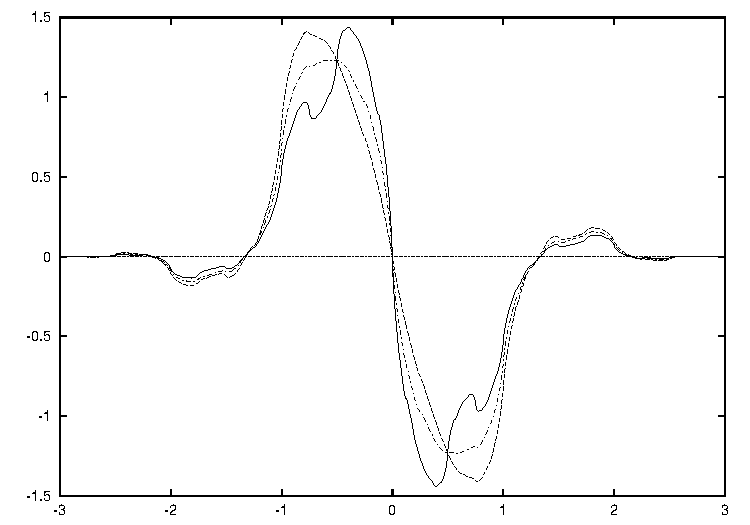
\includegraphics[  height=0.20\paperwidth,
  %keepaspectratio]{firstderivative_fund_-0_2_0_15_0}\end{center}


%\caption{\label{Figdifffund}Derivatives of the fundamental functions for
%$\alpha =-0.2$ (continuous line), $\alpha =0$ (dash-dot line), and
%$\alpha =0.15$ (dashed line). The fundamental functions are defined
%as the interpolation of $y_{0,k}=\delta _{k,0}$ by the HRS scheme
%initialized with the 4-point Deslauriers-Dubuc dyadic scheme. Derivatives
%were estimated using first-order forward finite differences after
%8 iterations of the HRS (discarding the placeholders at the last iteration).
%The $\alpha =0$ case is in fact the derivative of the Deslauriers-Dubuc
%fundamental function. The plot illustrates the fact that HRS interpolants
%are smooth (differentiable) for some values of $\alpha $.}
%\end{figure}


%
%************************ FIGURE ************************
%\midinsert
%\psone{lambdas.fig}{3.0}
%\figcaplong{\fn{FigLambdas}}{$HRS_{\alpha}$ is differentiable
%if $\lambda _{HR}(\alpha )=\max \left\{ \lambda _{1}(\alpha ),\lambda _{2}(\alpha )\right\} <1$}{0}
%\endinsert
%************************ FIGURE ************************

%\begin{figure}
%\begin{center}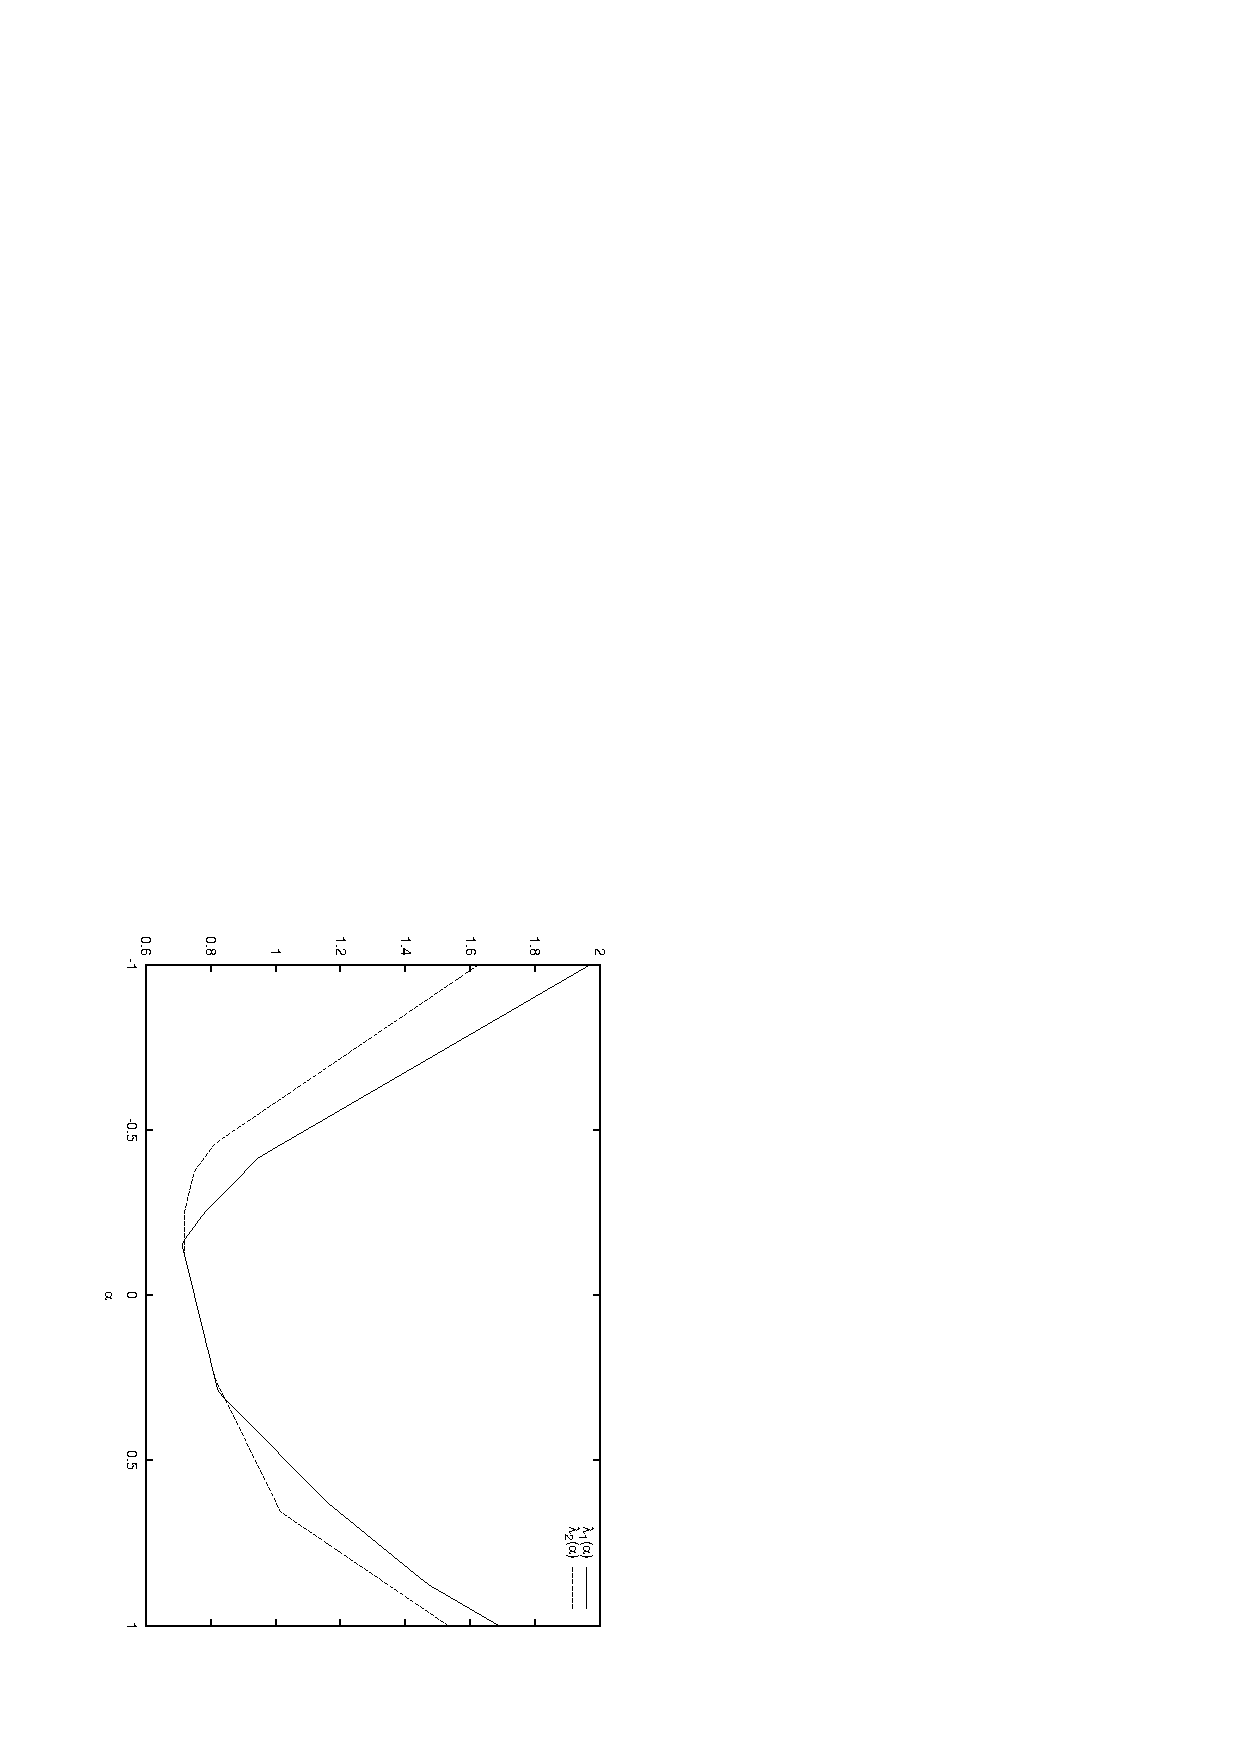
\includegraphics[  height=0.30\paperwidth,
  %keepaspectratio,
  %angle=270,
  %origin=c]{lambdas}\end{center}


%\caption{\label{FigLambdas}$\lambda _{1}(\alpha )$ (continuous line) and
%$\lambda _{2}(\alpha )$ (dashed line) as in the proof of theorem
%\ref{maintheorem}). For a given $\alpha $, a HRS scheme is differentiable
%if $\lambda _{HR}(\alpha )=\max \left\{ \lambda _{1}(\alpha ),\lambda _{2}(\alpha )\right\} <1$.}
%\end{figure}
%
%
%Given that the algorithm converges to continuous functions and is
%local, we can easily prove that it must be {}``stable''. In general
%terms, an algorithm $R$ is said to be stable if for any data $z$,
%$|R(z+\delta z)-R(z)|\leq K|\delta z|$ \cite{KuDa}.
%
%\proclaim Corrolary~\pn{corstable}. For $-25/56<\alpha <15/32$, the $HRS_{\alpha }$ 
%are stable, that is, given $\left|z_{j,k}-\widetilde{z}_{j,k}\right|<\delta \, \forall k\in \ZZ $
%then $\left|z_{j+n,k}-\widetilde{z}_{j+n,k}\right|<K\delta \, \forall k\in \ZZ $
%for all integers $n>0$ and a constant $K$ independent of $\delta $.
%
%\pf
%Assume we use any 4-point subdivision scheme as an initialization
%step on the initial data on $z_{j,k},\widetilde{z}_{j,k}$. For $-25/56<\alpha <15/32$,
%by theorem~\pr{maintheorem}, given the initial data $y_{j,k}=\delta _{k,0}\, \forall k\in \ZZ $,
%we get a continuous ($C^{1}$) interpolation function $F(x)$. Let
%$M=\left\Vert F\right\Vert _{L^{\infty }}$, assume $\left|z_{j,k}-\widetilde{z}_{j,k}\right|<\delta \, \forall k\in \ZZ $,
%by linearity, the interpolation function of $z_{j,k}-\widetilde{z}_{j,k}$
%is given by $f(x)=\sum _{k=-\infty }^{\infty }\left(z_{j,k}-\widetilde{z}_{j,k}\right)F_{j}\left(x-x_{j,k}\right)$
%but since $F$ has compact support $[x_{j,-3},x_{j,3}]$ then $\left\Vert f\right\Vert _{L^{\infty }}\leq 6M\delta $.
%It means that the values of the stable nodes are bounded by $-6M\delta $
%and $6M\delta $. The placeholders must also be bounded by $6M\delta \sum _{k\in \ZZ }\left|\gamma _{4k-1}^{DD4}\right|$(see
%equation~\er{hrswidguess}).
%\eop
  
  
  
  

%*************************** ACKNOWLEDGEMENTS ***********************

%\Acknowledgments{xxx}
  %% Replace xxx by your acknowledgement (if any)

%******************************* REFERENCES *************************

\References
  %%  Insert your references here
\rn{Dau}I. Daubechies, Orthonormal bases of compactly supported wavelets,
Comm. Pure \& Appl. Math. {\bf 41} (1988), 909--996.
\rn{DeDu}G. Deslauriers and S. Dubuc, Symmetric iterative interpolation processes,
Constr. Approx. {\bf 5} (1989), 49--68, .
\rn{DeDuLe}G. Deslauriers, S. Dubuc, and D. Lemire, Une famille d'ondelettes
biorthogonales sur l'intervalle obtenue par un sch�ma d'interpolation
it�rative, Ann. Sci. Math. Qu�bec {\bf 23} no. 1 (1999), 37--48.
\rn{DuGe}F. Dubeau and R. Gervais, Proc�dures locale et non locale d'interpolation
� l'aide de fonctions splines quadratiques, Ann. Sci. Math. Qu�bec
{\bf 23} no. 1 (1999), 49--61, 1999.
\rn{Du}S. Dubuc, Interpolation through an iterative scheme, J. Math. Anal.
Appl. {\bf 114} (1986), 185--204.
\rn{DuLeMe}S. Dubuc, D. Lemire, J.-L. Merrien, Fourier analysis of 2-point Hermite
interpolatory subdivision schemes, J. Fourier Anal.\ Appl. {\bf 7} no. 5 (2001).
\rn{Dyn}N. Dyn, Subdivision schemes in computer-aided geometric design, Advances
in numerical analysis (W. Light, ed.), vol. 2, Clarendon Press, 36--104, 1992.
\rn{DyGrLe}N. Dyn, J. A. Gregory, and D. Levin, A 4-point interpolatory subdivision
scheme for curve design. Comput. Aided Geom. Design {\bf 4} (1987), 257--268.
\rn{DynLevin}N. Dyn, D. Levin, Subdivision schemes in geometric modelling, Acta Numerica {\bf 12} (2002), 1--72.
\rn{Han2001}B. Han, Approximation Properties and Construction of Hermite Interpolants
and Biorthogonal Multiwavelets, J. Approx.\ Theory {\bf 110} no.1 (2001), 18--53.
\rn{HaIvDoSa}M. F. Hassan, I. P. Ivrissimitzis, N.A. Dodgson, and M.A. Sabin, An
Interpolating 4-Point $C^{2}$ Ternary Stationary Subdivision Scheme,
submitted for publication to CAGD (December 18, 2001).
\rn{HeilColella}C. Heil and D. Colella, Matrix refinement equations and subdivision
schemes, J. Fourier Anal. Appl. {\bf 2} (1996), 363--377.
\rn{KuDa}F. Kuijt and R. van Damme, Stability of subdivision schemes, Memorandum
no. 1469, Faculty of Applied Mathematics, University of Twente, the Netherlands.
\rn{Me92}J.-L. Merrien, A family of Hermite interpolants by bissection algorithms.
Numer. Algorithms {\bf 2} (1992), 187--200.
\rn{Me99}J.-L. Merrien, {\sl Interpolants d'Hermite $C^{2}$ obtenus par subdivision}.
M2An Math. Model. Numer. Anal. {\bf 33} (1999), 55--65.
\rn{Plonka}G. Plonka, {\sl Approximation order provided by refinable function vectors},
Constr. Approx. {\bf 13} (1997), 221--244.

%******************************* ADDRESS *************************

\Address
Daniel Lemire, Research Officer
National Research Council of Canada  (NRC) /
Conseil national de recherches du Canada (CNRC)
46 Dineen Drive
Fredericton, N.B.
E3B 5A3 Canada
{\tt lemire@ondelette.com}
{\tt http://www.ondelette.com/acadia/}


\bye
%% END of paper.tex
